\documentclass[english,12pt,a4paper,pdftex,sci,utf8]{./styles/aaltothesis}
\usepackage{graphicx}
\usepackage{ifpdf}
\ifpdf
   % put here packages only for the PDF:
   \DeclareGraphicsExtensions{.pdf,.png,.jpg,.mps}
   \usepackage{hyperref}
\else
   % put here packages only for the DVI:
\fi

% put all the other packages here:
\usepackage{./styles/clemens_thesis}

% \includeonly{./tex/preamble, ./tex/background }

\begin{document}

% !TEX root = ../thesis.tex
% !TEX spellcheck = en-US

\university{Aalto University}
\school{School of Science}

\department{Department of Information and Computer Science}
\professorship{Machine Learning, Data Mining, and Probabilistic Modeling}

\univdegree{MSc}

\author{Clemens Westrup}

%% Your thesis title comes here and again before a possible abstract.
%% If the title is very long and latex does an
%% unsatisfactory job of breaking the lines, you will have to force a
%% linebreak with the \\ control character.
%% Do not hyphenate titles.
%%
\thesistitle{From a fragmented process towards integrated end-to-end learning: An explorative study of the evolution of text classification approaches towards Deep Learning}

\place{Espoo}

\date{16.1.2015}

%% B.Sc. or M.Sc. thesis supervisor
%% Note the "\" after the comma. This forces the following space to be
%% a normal interword space, not the space that starts a new sentence.
%% This is done because the fullstop isn't the end of the sentence that
%% should be followed by a slightly longer space but is to be followed
%% by a regular space.
%%
\supervisor{Michael Mathioudakis, Ph.D.}

%% B.Sc. or M.Sc. thesis advisors(s). You can give upto two advisors in
%% this template. Check with your supervisor how many official advisors
%% you can have.
%%
\advisor{Prof.\ Aristides Gionis}
%\advisor{M.Sc.\ Polli Pohjaaja}

%% Aalto logo: syntax:
%% \uselogo{aaltoRed|aaltoBlue|aaltoYellow|aaltoGray|aaltoGrayScale}{?|!|''}
%%
%% Logo language is set to be the same as the document language.
\uselogo{aaltoYellow}{!}

%% Create the coverpage
%%
\makecoverpage

%% English abstract.
%% All the information required in the abstract (your name, thesis title, etc.)
%% is used as specified above.
%% Specify keywords
%%
%%
\keywords{NLP, bla bla, keyword}
%% Abstract text
\begin{abstractpage}[english]
  Your abstract in English. Try to keep the abstract short; approximately
  100 words should be enough. The abstract explains your research topic,
  the methods you have used, and the results you obtained.
  Your abstract in English. Try to keep the abstract short; approximately
  100 words should be enough. The abstract explains your research topic,
  the methods you have used, and the results you obtained.

  Your abstract in English. Try to keep the abstract short; approximately
  100 words should be enough. The abstract explains your research topic,
  the methods you have used, and the results you obtained.
  Your abstract in English. Try to keep the abstract short; approximately
  100 words should be enough. The abstract explains your research topic,
  the methods you have used, and the results you obtained.
\end{abstractpage}

%% Force a new page so that the possible English abstract starts on a new page
\newpage


%% Preface
\mysection{Preface}
I want to thank bla bla bla
\\

\vspace{5cm}
New York, 16.1.2015

\vspace{5mm}
{\hfill Clemens Westrup \hspace{1cm}}

%% Force new page after preface
%%
%% Pakotetaan varmuuden vuoksi esipuheen j�lkeinen osa
%% alkamaan uudelta sivulta
\newpage


%% Table of contents.
\thesistableofcontents


%% Symbols and abbreviations
\mysection{Symbols and abbreviations*}

% \subsection*{Symbols*}
%
% \begin{tabular}{ll}
% $\mathbf{B}$  & magnetic flux density  \\
% $c$              & speed of light in vacuum $\approx 3\times10^8$ [m/s]\\
% $\omega_{\mathrm{D}}$    & Debye frequency \\
% $\omega_{\mathrm{latt}}$ & average phonon frequency of lattice \\
% $\uparrow$       & electron spin direction up\\
% $\downarrow$     & electron spin direction down
% \end{tabular}

% \subsection*{Operators*}

% \begin{tabular}{ll}
% $\nabla \times \mathbf{A}$              & curl of vectorin $\mathbf{A}$\\
% $\displaystyle\frac{\mbox{d}}{\mbox{d} t}$ & derivative with respect to
% variable $t$\\[3mm]
% $\displaystyle\frac{\partial}{\partial t}$  & partial derivative with respect
% to variable $t$ \\[3mm]
% $\sum_i $                       & sum over index $i$\\
% $\mathbf{A} \cdot \mathbf{B}$    & dot product of vectors $\mathbf{A}$ and
% $\mathbf{B}$
% \end{tabular}

\subsection*{Abbreviations*}

\begin{tabular}{ll}
kNN & k-Nearest Neighbors \\
SVM & Support Vector Machine \\
NN & Neural Network \\
RNN & Recurrent Neural Network \\
LSTM & Long Short-Term Memory \\
MCC & Matthews Correlation Coefficient, see Section \ref{par:Informedness, Markedness and Matthews Correlation Coefficient}
\end{tabular}

\subsection*{Glossary*}
\begin{tabular}{ll}
one-hot-encoding & TODO \\
grid search & TODO \\
Crowdflower & TODO \\
Mturk & see \emph{Mechanical Turk} \\
Mechanical Turk & TODO \\
API & TODO \\
MongoDB & TODO \\
Mongoose & TODO \\
GitHub & TODO \\
\end{tabular}




%% Tweaks the page numbering to meet the requirement of the thesis format:
%% Begin the pagenumbering in Arabian numerals (and leave the first page
%% of the text body empty, see \thispagestyle{empty} below).
%% Additionally, force the actual text to begin on a new page with the
%% \clearpage command.
%% \clearpage is similar to \newpage, but it also flushes the floats (figures
%% and tables).
%% There is no need to change these
%%
\cleardoublepage
\storeinipagenumber
\pagenumbering{arabic}
\setcounter{page}{1}


\listoftodos

%\maketitle
%\tableofcontents
%\listoffigures
%\listoftables

%% Content
% !TEX root = ../thesis.tex
% !TEX spellcheck = en-US

%% Leave first page empty
\thispagestyle{empty}

% - what (problem statement)
% - why (need statement)
% - how (approach)
% - related
% - results

\section{Introduction}

Language is one of the most complex behaviors our species has developed. Humans use it to communicate even the most abstract concepts and it is considered one of the pillars of modern civilization. It takes children years to learn to communicate their thoughts and the subtle nuances of one's language give a glimpse one's cultural environment and upbringing, one's emotional state and one's intellect.

Not surprisingly in the field of Artificial Intelligence (AI) building computer systems with linguistic capabilities and solving language-based problems poses one of the hardest challenges and has motivated decades of research in Computational Linguistics. In fact many of the famous test for universal machine intelligence are based on linguistic capabilities, among them the famous \emph{Turing test} by~\cite{Turing:1950aa} where the task is for a human judge to determine whether he is having a conversation with a human or a machine in order to determine if the machine can be called intelligent, or the \emph{compression test} proposed by~\cite{Mahoney:1999aa}, where a human's and machine's capability to predict missing words given a context is tested.

This thesis explores the specific task of predicting the semantic structure of job advertisements as a specific example of such a language-based task that turns out to be difficult even for humans to do.
The work was done in close collaboration with the Helsinki-based media and learning company \emph{Sanoma}\footnote{\textquote{Sanoma is a front running consumer media and learning company in Europe. In Finland and the Netherlands we are the market leading media company with a broad presence across multiple platforms. In Belgium we are among the Top 5. Our main markets in learning are Belgium, Finland, the Netherlands, Poland and Sweden. We entertain, inform, educate and inspire millions of people every day. We employ some 7,500 professional employees operating in Europe.}, Source: \url{http://www.sanoma.com/en/who-we-are}, visited 06.06.2016} and the research motivation was thus constantly tied back into real world challenges in the scope of Sanoma's business needs.



\subsection{Need Statement and Motivation}

Today's media and education, the basis of Sanoma's core businesses, are undergoing drastic and fundamental transformations that are currently disrupting whole industries.

Usage of digital media as a source of information has long surpassed print media. Sanoma's most well-known product, Finland's biggest daily newspaper \emph{Helsingin Sanomat}, lost 6\% of its circulation only in 2015\footnote{Source: http://www.digitalnewsreport.org/survey/2016/finland-2016/, visited 27.07.2016}, while the wide-spread use of social media challenges traditional ways we access information. Similarly in the field of education, with the rise of Massive open online course (MOOCs), traditional learning settings are challenged and the need for advanced techniques for data processing and analysis increases, e.g.\ to personalize and adapt the learning experience to each individual user and at the same time identify trends across large groups of learners to better meet the needs of education.

Sanoma provides a recruitment platform named \emph{Oikotie Työpaikat}. The service is in direct competition several other international players in the recruitment industry. Through this and other services Sanoma's collects large amounts of user-generated data, offering the potential to be leveraged for machine learning solutions to provide value for their users and innovate and enrich the company's offerings.
This was the company's initial motivation for this thesis project --- To explore ways to leverage user-generated data to potentially.

From my perspective this offered many interesting research possibilities while at the same time being relevant for a real business. Natural Language Processing and Computer Linguistics had always been of strong interest to me for the complex nature and yet high interpretability of problems and their proximity and relatedness to progress in universal machine intelligence. This presented me with the challenge position to balance pursuing research objectives and yet exploring potential business and user needs, learn on new fronts and deepen my knowledge in others as well as combining my experience in Product Innovation, thus made for a great project to mark the competition of my studies as a Master's student.

\subsection{Problem Statement}

The problem addressed during with this thesis to better understand the structure of job advertisements. In particular job postings typically consist of several parts with a certain function or theme: Usually company is introduced, the job is described with it's tasks and responsibilities, the requirements for the job are listed, then benefits and offerings by the company are named and the reader is asked to apply in a specified way he or she is interested.
Almost all of the text\footnote{Only 4\% of the sentences collected for evaluating the final experiments in this thesis were sorted into the category \emph{other} while the rest falls into either of the categories described. This is described in more detail in Section }\todo{link section} of a job description falls into these categories and the task can thus be posed as predicting a category for each sentence in a job advertisement, that corresponds with this sentence belonging to one of the job ads' parts as described above.
This is a challenging problem in itself but can further be used to extract certain functional parts of each job ad, to study a possible correlation between structural patterns and the reach and success of an ad and so forth. The problem therefore can be labelled as \emph{Text Categorization} or \emph{Text Classification} as referred to in the scientific literature.

\subsection{Related work *}

The research problem of Text Classification is one of the various challenges in the thriving fields of Computational Linguistics (CL) and Natural Language Processing (NLP). These areas of research have started out as theoretically challenging but rather marginally interesting fields between Artificial Intelligence (AI) and formal linguistics and have since exploded in terms of popularity with their applications being deployed nowadays at large scale to practically all kinds of consumer electronics such as smart phones and home entertainment systems as well as disrupting whole industries e.g.\ by replacing human workforce with conversational agents where applicable.
Today there are several textbooks dedicated specifically to this area, such as~\cite{Manning:1999aa},~\cite{Jurafsky:2014aa} and~\cite{Clark:2013aa} as well as much overlap in the field of Information Retrieval (IR) that rose to popularity during the late 1980's due to the Internet starting to become a mainstream medium (see~\cite{Manning:2008aa},~\cite{Leskovec:2014aa} and the classic work by~\cite{Rijsbergen:1979aa}).

The field of Natural Language Processing has undergone different trends of modeling approaches since its beginnings that~\cite{Cambria:2014aa} identities as three main curves of \emph{Syntactics}, \emph{Semantics}, and \emph{Pragmatics}. The The first trend of syntax-centered NLP is still prevalent and is based on algorithms that more or less directly operate on the words found in the processed texts.
The second trend operates on the semantics of text, thus being able to potentially tackle more challenging problems by addressing increasingly subtle notions of meaning and context. According to the author these types of approaches are still in the early phase but at the verge of being adapted by a broader audience of researchers and practitioners in the field. The last trend curve of pragmatics a yet more complex issue of modeling inherent narratives in language where so far only pioneering work has been done but which, according to the author, will lead to tackling problems of natural language understanding. This thesis falls between the first and second trend curve by comparing more traditional, syntax based approaches to those modeling latent semantics.

The problem of Text Categorization specifically has seen a tendency of following these trends loosely. The task itself has been of immense interest for several decades now due to the exponentially increasing amounts of text data being recorded with the dawn of user generated content through social networks etc. and increased digitalization of our daily lives. Its applications reach from document filtering, automated metadata generation such as language classification to automatic email labeling, spam identification and sentiment detection, amongst others.

It is \cite{Sebastiani:2002aa} points out it is important to mention that the term \emph{automatic text classification} has also been used referring to different problems: \textquote{Aside from (i) the automatic assignment of documents to a predefined set of categories, which is the main topic of this paper, the term has also been used to mean (ii) the automatic identification of such a set of categories (e.g., [\cite{Borko:1963aa}]), or (iii) the automatic identification of such a set of cat- egories and the grouping of documents under them (e.g., [\cite{Merkl:1998aa}]), a task usually called text clustering, or (iv) any activity of placing text items into groups, a task that has thus both TC and text clustering as particular instances [\cite{Manning:1999aa}]}~\cite{Sebastiani:2002aa}

Early approaches towards solving text classification tasks in the 1980's were in often based on expert systems consisting of sets of manually created logical rules, deciding upon the category of a text segment if a certain formula applies. As discussed by \cite{Sebastiani:2002aa} the biggest downside is known as the \emph{knowledge acquisition bottleneck} which refers to the fact that each rule has to be manually created. In the 1980's machine learning approaches became more common where a \emph{classifier} is learns the attributes of the data and its association with the given data labels using a model that allows to then infer the categories for unseen data. This setting is called \emph{supervised learning} as labels for the data are given and are aimed to be predicted.

Machine learning approaches have since been developed in countless variations. Most follow a classical pipeline of \emph{feature extraction} or \emph{indexing} of documents followed by \emph{inductive construction} of a classifier that is lastly evaluated by a measure of effectiveness. A very successful approach to feature extraction has been the introduction of N-Gram based models, also called \emph{bag-of-words} models since they are more or less insensitive to the order of the words depending on the window size of the cooccurrence statistics chosen. These exist in a variety of forms and are based on word-cooccurrence frequencies of the terms that are present in the data. Various techniques exist for dimensionality reduction or feature selection of these models as well as certain smoothing techniques (refer to Section~\ref{subs:N-gram Models} for an in-depth introduction).


% ## related fields
%
% # NER
% \cite{Baluja:2000aa} - Applying Machine Learning for High-Performance Named-Entity Extraction
% \cite{Zhang:2004aa} - Zhang-Focused Named Entity Recognition Using
% \cite{Strzalkowski:1996aa} - A Self-learning Universal Concept Spotter
% \cite{Alfonseca:2002aa} - An unsupervised method for general named entity recognition and automated concept discovery
% \cite{Nadeau:2007aa} - A survey of named entity recognition and classification.
%
% # Topic modeling
% \cite{Blei:2012aa} - Probabilistic Topic Models
%
%
% # Ngram models
% \cite{Jagadish:1998aa} - Optimal histograms with quality guarantees
%
% # language modeling
% \cite{Bengio:2006aa} - Neural Probabilistic Language Models.
% \cite{Mikolov:2013aa} - Exploiting similarities among languages for machine translation.
% \cite{Mikolov:2012aa} - Statistical Language Models Based on Neural Networks
%
%
%
% # CNNs
% \cite{Kim:2014aa} - Convolutional neural networks for sentence classification
% \cite{Cheng:2014aa} - Investigating the role of prior disambiguation in deep-learning compositional models of meaning
% \cite{Kalchbrenner:2014aa} - A convolutional neural network for modelling sentences
% \cite{Johnson:2014aa} - Effective Use of Word Order for Text Categorization with Convolutional Neural Networks
%
%
%
% # sequential modeling
% \cite{Lafferty:2001aa} - Conditional Random Fields: Probabilistic Models for Segmenting and Labeling Sequence Data
%
% # \cite{Lewis:1992aa} - Feature selection and feature extraction for text categorization
%
%
% Unsupervised techniques for topic discovery have been investigated widely, such as LSA
%
% Vector Space models are a
%
% - feature learning for text
% - multitask learning
%
% \cite{Bastian:2014aa} - ontology learning, topic extraction approach
%
%
% \cite{Collobert:2008aa} showed how both multitask learning and semi-supervised learning improve the generalization of the shared tasks on text data. They describe \textquote{a single convolutional neural network architecture that, given a sentence, outputs [\ldots] part-of-speech tags, chunks, named entity tags, semantic roles, semantically similar words and the likelihood that the sentence makes sense (grammatically and semantically) using a language model}.
%
% \cite{Lodhi:2002aa} string kernels
%
% \todo{section on transfer learning and feature learning}
% \todo{text classification}
% \todo{Multitask learning}
% \todo{explicit vs implicit feature representation}


\subsection{Research Objectives and Scope *}


- study vector space models and new approaches
- study sequential and multi-task approaches
- mu

\subsection{Approach *}

asd

\subsection{Results *}

asdasd

\subsection{Structure of the thesis @}

The first section of this thesis gave a brief introduction into the topic of this work, outlined the motivation and the research problem approached and showed the research objectives, the scope of the thesis as well as related work.

Section~\ref{sec:Background}:~\nameref{sec:Background} introduces the reader to concepts and ideas of Text Classification in order to provide him or her with the necessary knowledge to understand the work described in this thesis. First the problem of Text Classification is formally defined and the most common approaches to this problem are described on a high level. Afterwards Vector Space Models are introduced in detail, which represent a popular way of tackling this task by transforming text into fixed-size vectors.
The following subsection then briefly presents several of the most known classification algorithms that can operate on the vectors produced by such Vector Space Models. Next the approach of Sequential Classification is described in short where text is treaded as a one-dimensional signal in time. The following subsection then shows common ways to evaluate how well the task of text classification is solved and the last subsection gives a brief introduction to two methods that are useful for exploring different models and techniques through visualization.

Section~\ref{sec:Exploration}:~\nameref{sec:Exploration} gives an overview of the exploration of the wider topic space at the start of the thesis project as well as the experimentation with different techniques and the data given for the project. It aims to lay out to the reader the process, insights and learnings leading towards the final problem formulation and evaluation of methods to solve this problem.

The following Section~\ref{sec:Experimental Evaluation of Multi-class Prediction of Semantic Categories for Text in Job Advertisements}:~\nameref{sec:Experimental Evaluation of Multi-class Prediction of Semantic Categories for Text in Job Advertisements} then presents the main results of the thesis. The exact problem definition is given that is used as a basis to evaluate the experiments and the dataset used for these experiments is described.
Subsequently the evaluation of the different approaches to Vector Space Models, the classification algorithms using the most successful of these models and the sequential modeling approach are documented. Each of these subsections first describes the experimental setup, followed by results of the different approaches and closes with a brief discussion on the outcomes presented.

% !TEX root = ../thesis.tex
% !TEX spellcheck = en-US

\clearpage

\section{Background}
\label{sec:Background}

This chapter will provide the necessary background on text classification, assuming the reader is familiar with the basic concepts of Machine Learning and related fields. First the research problem will be defined. Then

\subsection{Text classification}
\label{sub:Text classification}

\subsubsection{Problem Formalism}
\label{subs:Problem Formalism}

Text classification, also known as text categorization, is the task of predicting a \emph{mapping} $\widetilde{\Phi} : \mathcal{D} \times \mathcal{C} \rightarrow \{True, False\}$ between a set of documents $\mathcal{D}$ and a set of classes or categories $\mathcal{C}$ using a model function $\Phi : \mathcal{D} \times \mathcal{C} \rightarrow \{True, False\}$. This means that were are trying to predict as good as possible the categories that each document belongs into, or vice versa the documents associated with each category. This mapping can thus be represented as a bipartite graph between the sets of documents $\mathcal{D}$ and categories $\mathcal{C}$ as shown in Figure~\ref{fig:bipartite-graph-text-classification}. In this representation vertices in the graph indicate a $True$ value in the mapping, indicating that the document and category are associated with each other, while missing vertices indicate that they are not ($False$).

\begin{wrapfigure}{r}{0.5\textwidth}
  \begin{center}
    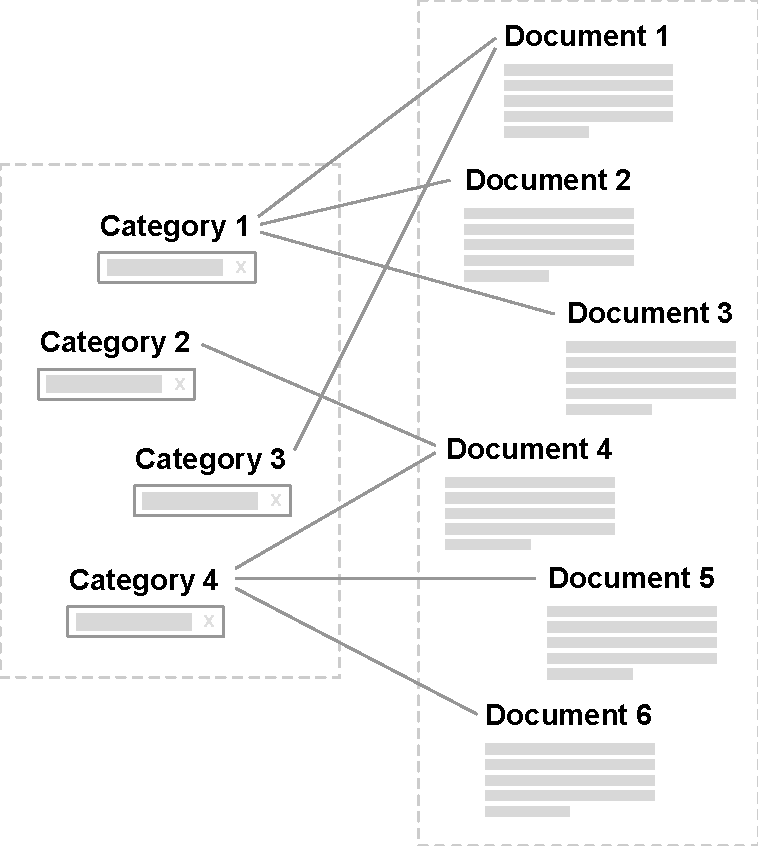
\includegraphics[width=0.5\textwidth]{img/bipartite-graph-text-classification}
  \end{center}
  \caption{Text classification visualized as a bipartite graph. Here the multi-label setting is shown where no additional constraints are enforced on the problem and hence each document can be assigned to multiple categories}
\label{fig:bipartite-graph-text-classification}
\end{wrapfigure}

Categories $\mathcal{C}$ are given as symbolic labels and documents $\mathcal{D}$ as chunks of text with variable length. We usually assume that no additional information such as metadata or other \emph{exogenous knowledge} is available on neither labels nor documents.
As~\cite{Sebastiani:2002aa} points out a consequence of relying solely on \emph{endogenous knowledge}, especially the semantics of a text, is that there is no objective ground truth to this task in most settings since semantics are a \emph{subjective} notion: \textquote{This is exemplified by the phenomenon of inter-indexer inconsistency [Cleverdon 1984]\todo{reference}: when two human experts decide whether to classify document $d_j$ under category $c_i$, they may disagree, and this in fact happens with relatively high frequency. A news article on Clinton attending Dizzy Gillespie’s funeral could be filed under Politics, or under Jazz, or under both, or even under neither, depending on the subjective judgment of the expert.}~\cite{Sebastiani:2002aa}

Additional constraints can be imposed on the problem to adapt it for different application scenarios. Firstly text classification can be either framed as \emph{single-label} classification where each document is assigned to only one single category or \emph{multi-label} classification where an assignment to several categories or also no category is possible. The multi-label case can also be formulated as $|\mathcal{C}|$ individual binary classification problems which of course assumes statistical independence between these prediction tasks.

In order to measure how successfully we are tackling the problem of text classification we need metrics that measure the effectiveness of our algorithm given a dataset. These will be discussed in Section~\ref{sub:Evaluation}.

\subsubsection{Approaches to Text Classification *}

% \subsubsection{Text as a Sequential Signal}
% \label{par:Text as a Sequential Signal}

% Text can be seen as a sequential signal like any other. Depending on the task at hand the resolution of this signal can be chosen more or less fine-grained, ranging from single characters to words, sentences, paragraphs or whole documents. The more fine-grained we choose our model to operate, the more sequential correlation we usually find, as characters, words tend to follow linguistic rules that constrain in which order combinations they can be used, and even sentences and paragraphs are often semantically related. This observation motivates the use of language models for the text classification task as will be discussed in Section \todo{reference}.

\subsection{Vector Space Models *}

Text documents cannot be used directly as input to a classifier, and are thus usually mapped into a vector space so that each document can be represented by a vector $\mathbf{v} \in \mathbb{R}^d$. This procedure is also known as \emph{Document Indexing}~\cite{Sebastiani:2002aa}.


\textquote{Contiguity hypothesis. Documents in the same class form a contiguous region and regions of different classes do not overlap.}~\cite[Chapter 14, p.~289]{Manning:2008aa}

Vector space model~\cite[Chapter 6.3, p.~120]{Manning:2008aa}

\textquote{the document `Mary is quicker than John' is, in this view, identical to the document `John is quicker than Mary'}\cite[Chapter 6.2, p.~117]{Manning:2008aa}


\subsubsection{N-gram Models}
\label{subs:N-gram Models}

N-gram language models are based on co-occurrences of word or character sequences, so-called N-grams or $k$-shingles as they are referred to in the Data Mining literature~\cite[Chapter 3.2, p.~72]{Leskovec:2014aa}. Formally an N-gram is defined as a sequence of $n$ items, each of which consist of $n$ characters or words, effectively used to capture sub-sequences of text. Common choices are N-grams of size 1, 2 or 3 --- called \emph{unigrams}, \emph{bigrams} and \emph{trigrams} respectively --- and the definition can be extended to using a window size $[\textit{w}_{\text{min}}, \textit{w}_{\text{max}}]$, employing all combinations of N-grams in this interval.

N-grams are usually used to create a vector-space model by representing each document in a dataset as a \textit{bag-of-words} or \textit{bag-of-N-grams} vector so that each dimension of the vector represents statistics about the corresponding N-gram. Specifically, a common way to compute the word count vectors for a document is the following:

\begin{equation}
  \text{TF}_{ij} = \frac{f_{ij}}{\max_k f_{kj}}
\end{equation}

Where $f_{ij}$ is \textquote{the \emph{frequency} (number of occurences) of a term (word) $i$ in document $j$} and $\text{TF}_{if}$ is the \emph{term frequency}, i.e.   \textquote{$f_{ij}$ normalized by dividing it by the maximum number of occurrences of any term [\ldots] in the same document}~\cite[Chapter 1.3.1, p.~8]{Leskovec:2014aa}.

\todo{example with 2 vectors and showing what they encode?}

\paragraph{Variants}

As this approach has been studied for decades \todo{citation for first or review paper here?} there is quite an extensive amount of variants and thus hyper-parameters to tune. The most important ones will be explained in the following sections:

\subparagraph{Words vs. Characters} The first choice when building an N-gram language model is to use characters or words as the atomic unit. In practically every case there are less characters than words in a dataset, but to capture expressive substrings usually larger N-gram window sizes or ranges have to be chosen, which leads to a combinatorial explosion. In case of word-based models on the other hand the maximal size of the feature space is the size of the vocabulary $\mathcal{V}$ in the case of unigrams or $V^k$ in case of $k$-grams.

\subparagraph{Stop words}
\label{subp:Stop words}
For creating N-gram models, so-called stop word lists are often used which are lists of frequent words that will be excluded as they do not carry much meaning~\cite[Chapter 1.3.1, p.~7]{Leskovec:2014aa}. The stop-word list used in these experiments is the standard list used for the Scikit-learn framework~\cite{Pedregosa:2011aa} which is a list gathered by the University of Glasgow Information Retrieval group\footnote{\url{http://www.gla.ac.uk/schools/computing/research/researchoverview/informationretrieval/}. The full stop word list can be found at \url{http://ir.dcs.gla.ac.uk/resources/linguistic_utils/stop_words} and in the appendix in Section~\ref{sec:appendix-stopwords}.}.

\subparagraph{N-gram range} The N-gram range, also known as window size or shingle size, refers to combinations of the atomic units of the model (words or characters) and defines an upper and lower limit for these combinations. For example a range of $[1,1]$ specifies a unigram model, $[2,2]$ a bigram model and $[1,2]$ a combination of both including all unigrams and all bigrams.
A larger range allows the model to capture an increasing amount of word order and thus context, but again leads to a combinatorial explosion in terms of feature space.

\subparagraph{Vector size} The vector size imposes an upper limit to the vector size and therefor the number of N-grams that can be encoded in the feature space. Commonly this simply uses the words with the highest frequency to reduce the vector size from the full length --- the size of the vocabulary --- to the desired size.

\subparagraph{TF.IDF weighting}
\label{subp:TF.IDF weighting}
A common extension to using word-counts is to weight the term frequencies by the so-called inverse document frequency, i.e.\ the inverse of the frequency of an term or N-gram in all documents. This method is commonly referred to as \emph{TF.IDF} and specifically the inverse document frequency is defined as $\text{IDF}_i = \log_2 (N/n_i)$, where logarithmic smoothing is applied. The TF.IDF value for a term or N-gram is then computed as $\text{TF}_{ij} \cdot \text{IDF}_i$.

\subparagraph{Sublinear TF scaling}
\label{subp:Sublinear TF scaling}
 As~\cite[Chapter 6.4.1, p.~126]{Manning:2008aa} suggests \textquote{[it] seems unlikely that twenty occurrences of a term in a document truly carry twenty times the significance of a single occurrence}. Hence a common variant is \emph{sublinear scaling} where we down-weigh the increase in term importance by applying a logarithmic function to it, resulting in the sub-linear term frequency $\text{subTF}_{ij}$:

\begin{displaymath}
  \text{subTF}_{ij} = \left \{ \begin{array}{l l} 1+\log \text{TF}_{ij} & \text{TF}_{ij} > 0 \\
  0 & \text{otherwise}
\end{array} \right \}
\end{displaymath}

\subparagraph{Normalization} Often the term vectors are globally normalized using the $L_1$ or $L_2$ norm to remove the effect of statistical differences between the terms.

There are, of course, various other variants and modifications to the N-gram model, but within the scope of this thesis only the most notable ones were introduced and will be used for experiments later. For further material on this subject refer for example to~\cite{Manning:2008aa}.

\todo{mention smoothing techniques~\cite{Chen:1996aa}}

\paragraph{Shortcomings}
\label{subs:shortcomings-ngrams}

Today N-gram models are still in wide use and considered as state of the art \textquote{not because there are no better techniques, but because those better techniques are computationally much more complex, and provide just marginal improvements}~\cite[p.~17]{Mikolov:2012aa}. As~\cite{Mikolov:2012aa} points out further \textquote{[the] most important weakness is that the number of possible n-grams increases exponentially with the length of the context, preventing these models to effectively capture longer context patterns. This is especially painful if large amounts of training data are available, as much of the patterns from the training data cannot be effectively represented by n-grams and cannot be thus discovered during training. The idea of using neural network based LMs [Language Models] is based on this observation, and tries to overcome the exponential increase of parameters by sharing parameters among similar events, no longer requiring exact match of the history H.}~\cite[p.~17]{Mikolov:2012aa}

\subsubsection{Language Models using Distributed Representations @}
\label{subs:Language Models using Distributed Representations}


\begin{wrapfigure}{r}{0.5\textwidth}
  \begin{center}
    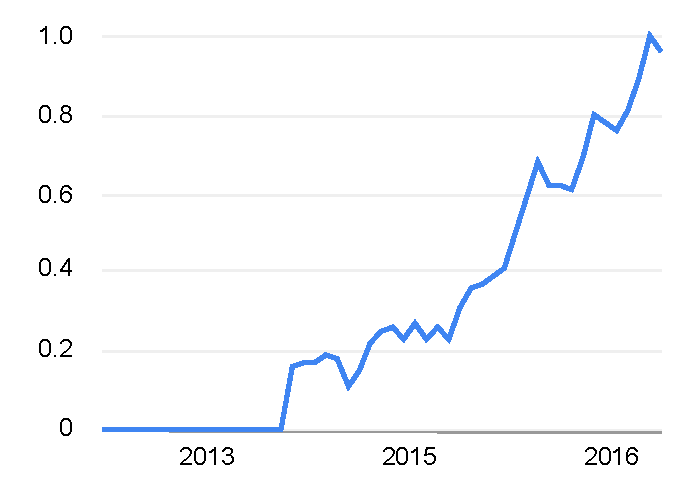
\includegraphics[width=0.48\textwidth]{img/word2vec-google-trends.pdf}
  \end{center}
  \caption{Google Trends statistics on relative search interest in the term ``word2vec''. Retrieved on 22.05.2016.}
\label{fig:word2vec-google-trends}
\end{wrapfigure}

To overcome the shortcomings of popular language models such as the ones of the N-gram model mentioned above, lots of recent work went into the study of so-called distributed language models. One branch of research that gained significant attention is the work on Neural Network based Language models (NNLMs), popularized largely through the work of T. Mikolov and his software realization of such a model dubbed \emph{word2vec} with interest coming not only from the academic community but also from open source community (Figure~\ref{fig:word2vec-google-trends} shows the search relevance of the term ``word2vec'' in the recent years). His work builds on ideas introduced in~\cite{Bengio:2000aa} where a neural network based model was proposed for modeling high-dimensional discrete data, which was then applied to the domain of language modeling in~\cite{bengio2003neural}. Following the description in this paper, the approach is as follows:

\begin{enumerate}
  \item Associate with each word in the vocabulary a distributed \emph{word feature vector} (a real-valued vector in $\mathbb{R}^m$),
  \item Express the joint \emph{probability function} of word sequences in terms of the feature vectors of these words in the sequence, and
  \item Learn simultaneously the \emph{word feature vectors} and the parameters of that \emph{probability function}.
\end{enumerate}

To achieve this, a feedforward neural network model is trained to learn these \emph{word feature vectors} or \emph{word embeddings}. As input a sequence of $n$ words is given, each encoded using one-hot encoding or one-of-$V$ encoding where the corresponding indicator vectors for each word have the size of the vocabulary $V$. The input word vectors are then projected linearly into a projection layer of significantly lower dimensionality $D$, using a global projection matrix for across all words, and concatenated, forming the input of size $D \times N$ to a hidden layer of size $H$. The hidden layer then feeds non-linearly into the output layer that is again of size $V$, modeling the probability distribution for a word given its context $P(w_t \mid w_{t - n}, \ldots, w_{t - 2}, w_{t - 1})$.

\paragraph{Simplified Continuous Models}

\cite{Mikolov:2013ad} then introduced two simplified models, removing the hidden layer and only using a projection layer, with shared weights for all words. The Continuous Bag-of-Words Model (CBOW) model is trained to predict the current word $w_t$ given the $k$ words around it. Its name is due to the fact that the word order does not influence the projection as the word vectors are summed or averaged. The Continuous Skip-gram Model works the other way around, predicting the most likely $k$ words around a given word $w_t$. Figure~\ref{fig:cbow-skip-gram} illustrates both models.

\begin{figure}[h]
    \centering
    \begin{subfigure}[b]{0.49\textwidth}
        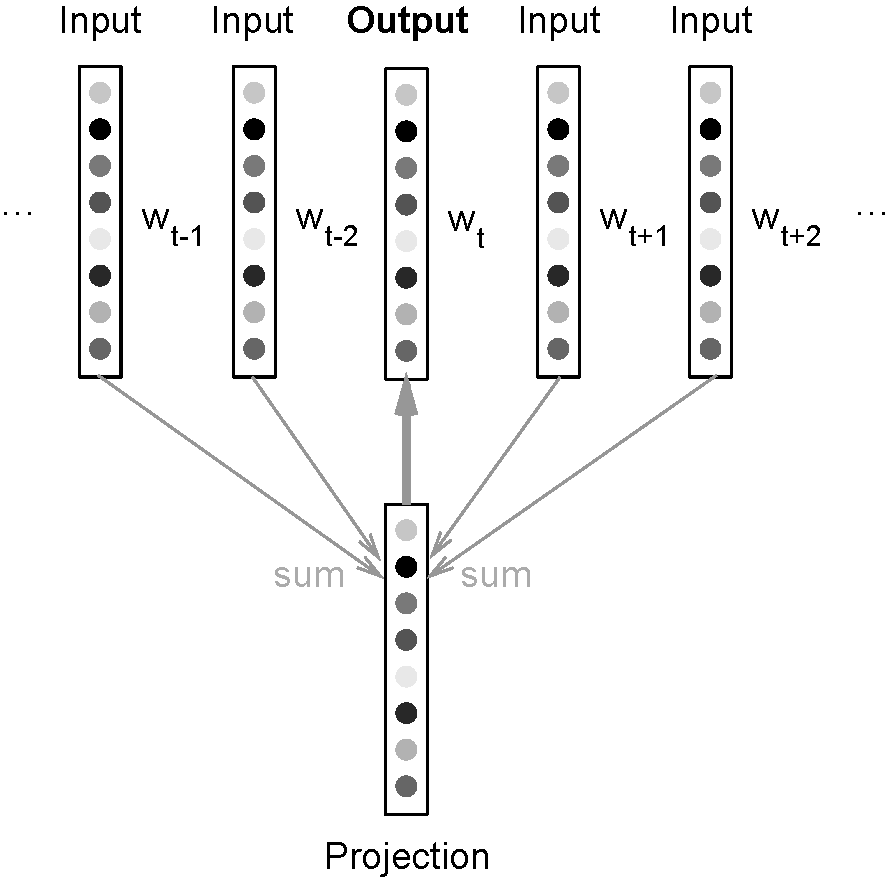
\includegraphics[width=\textwidth]{img/cbow_vert2.pdf}
        \caption{Continuous Bag-of-Words Model}
\label{fig:cbow}
    \end{subfigure}
    %add desired spacing between images, e. g. ~, \quad, \qquad, \hfill etc.
      %(or a blank line to force the subfigure onto a new line)
    \begin{subfigure}[b]{0.49\textwidth}
        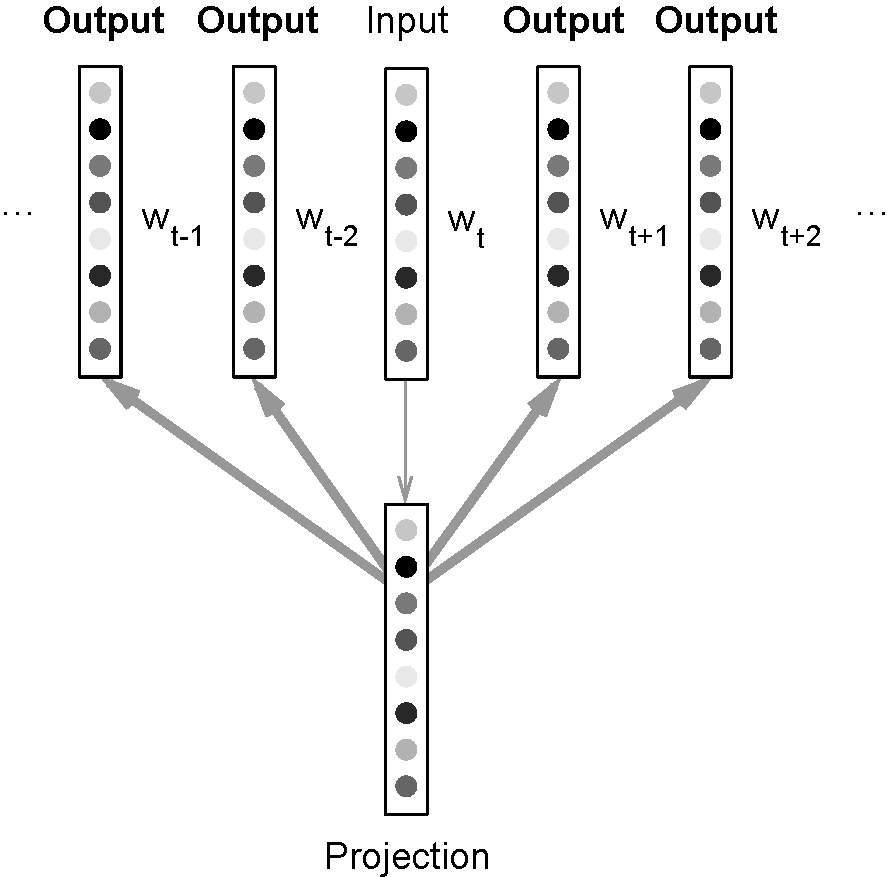
\includegraphics[width=\textwidth]{img/skip-gram_vert2.pdf}
        \caption{Continuous Skip-gram Model}
\label{fig:skip-gram}
    \end{subfigure}
    \caption{Architectures for learning continouus distributed word vectors, adapted from~\cite{Mikolov:2013ad}}
\label{fig:cbow-skip-gram}
\end{figure}

\begin{wrapfigure}{l}{0.6\textwidth}
  \begin{center}
    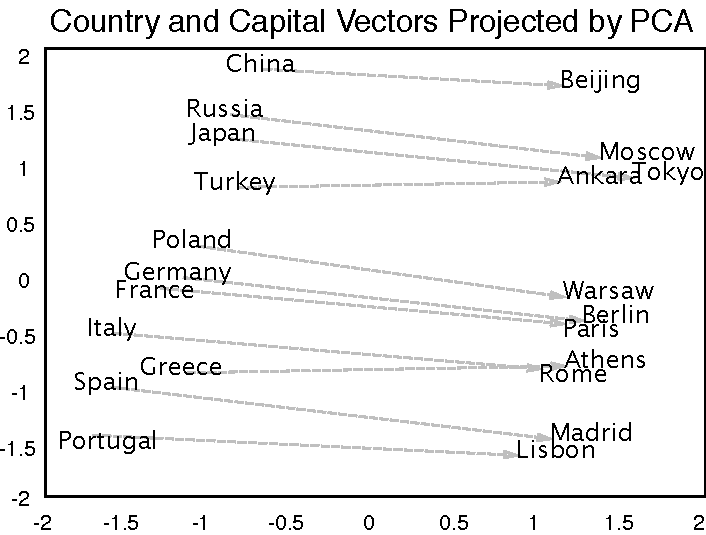
\includegraphics[width=0.58\textwidth]{img/word2vec_cities.pdf}
  \end{center}
  \caption{Two-dimensional PCA projection of the 1000-dimensional Skip-gram vectors of countries and their capital cities. The figure illustrates ability of the model to automatically organize concepts and learn implicitly the relationships between them, as during the training we did not provide any supervised information about what a capital city means. (Adapted from~\cite{Mikolov:2013ac})}
\label{fig:word2vec-cities}
\end{wrapfigure}

These models have been shown to outperform state of the art N-gram models on various tasks (see e.g.~\cite{bengio2003neural} or~\cite{Mikolov:2012aa}). An interesting outcome of this research is the fact that these \emph{word vectors} capture many interesting and often subtle semantic regularities and that these can be exploited explicitly in an algebraic manner. When trained on an extensive dataset, one can perform calculations as $v(Paris) - v(France) + v(Germany)$ and the closest vector to the result turns out to be $v(Berlin)$ where $v(\cdot)$ denotes the \emph{word vector} of a word. Figure~\ref{fig:word2vec-cities} shows a PCA projection of Skip-gram trained vectors of countries and their capital cities.

A notable alternative to these models was developed by~\cite{Pennington:2014aa}. In their model called \emph{GloVe}, which stands for global vectors, they construct a vector space model with similar properties as the models introduced above, which instead relies global word-word co-occurrence counts. This method thus operates directly in the co-occurrence statistics of the corpus compared to the Neural Network based methods that \textquote{fail[\ldots] to take advantage of the vast amount of repetition in the data}~\cite{Pennington:2014aa}.

There have been various extensions and variants to the Neural Network based language models especially, including architectures based on Recurrent Neural Networks (see~\cite{Mikolov:2012aa}). Some of the most important variations will are discussed in the following section as they were evaluated in the experiments:

\subparagraph{Hierarchical Softmax}
The architectures proposed in~\cite{Bengio:2000aa},~\cite{bengio2003neural} and follow-up work use a \emph{softmax} activation function at the output layer in order to obtain valid probabilities for each word to be predicted:

\begin{equation}
  \operatorname{softmax}(\mathbf{x}_j) = \frac{\exp(\mathbf{x}_j)}{\sum_k \exp(\mathbf{x}_k)}
\end{equation}

\emph{Hierarchical Softmax} uses a binary tree to encode the output which leads to an efficient approximation of the full softmax and speeds up training and inference. Details can be found in~\cite{Mikolov:2013ab}.

\subparagraph{Negative Sampling}
Another technique applied by~\cite{Mikolov:2013ab} \emph{Negative Sampling} which is a simplified version of Noise Contrastive Estimation (NCE) introduced by~\cite{Gutmann:2012aa}. Based on the insight that a good model should be able separate noise from signal, this method mixes samples from a noise distribution into the signal to be learned, in this case random words that are not in the context window, which is shown to approximately maximize the log probability of the softmax. Free parameters of this technique are the number of negative samples $k$ per data sample and the noise distribution $P_n(w)$

\subparagraph{Sub-sampling of Frequent Words}
As there the difference between frequent and infrequent words in large corpora can be huge and the frequent words often don't carry as much meaning, in~\cite{Mikolov:2013ab} a simple sub-sampling technique is used to counter this imbalance by discarding words with a probability computed as follows:

\begin{equation}
  P(w_i) = 1 - \sqrt{\frac{t}{f(w_f)}}
\end{equation}

with $f(w_i)$ denoting the frequency of word $w_i$ and $t$ denoting a threshold.~\cite{Mikolov:2013ab} state that this method, while chosen heuristically, \textquote{accelerates learning and even significantly improves the accuracy of the learned vectors of the rare words}.

\paragraph{Distributed representations for documents}
\label{par:Distributed representations for documents}

The models explained above are defined on words as the atomic unit. Therefore several ways have been proposed to extend these to sequences of words in order to obtain a vector space of sentences or documents. A few of these will be briefly outlined here:

\subparagraph{Bag-of-Means}
\label{subp:Bag-of-Means}
The term \emph{Bag-of-Means} refers to simply averaging over the word embedding vectors of all words in a document. However this approach \textquote{loses the word order in the same way as the standard bag-of-words models do.}~\cite{Le:2014aa}. This intuitive property was confirmed by~\cite{Zhang:2015aa} where the method consistently performed poorest in comparison to other approaches on a variety on tasks.

\subparagraph{Parse Trees}~\cite{Le:2014aa} also mention a more sophisticated approach by \textquote{combining the word vectors in an order given by a parse tree of a sentence.} as done in~\cite{Socher:2011aa}, with the disadvantage that this method \textquote{has been shown to work for only sentences because it relies on parsing}~\cite{Le:2014aa}.

\subparagraph{Paragraph Vectors *}
In~\cite{Le:2014aa} a different approach is shown that builds on the same idea as the original word2vec model:

\subsection{Classification Algorithms for Vector Space Models *}
\label{sub:Classification Algorithms for Vector Space Models}

\paragraph{Classification Schemes}
\label{par:Classification Schemes}
As will be discussed later in Section~\ref{sub:Evaluation}, there are three common schemes for classification: In \emph{binary classification} there is only a single class and for each document we decide whether or not it belongs to this class. A classic example is email spam detection where we predict if a given email is spam or not. \emph{Multi-class classification} assumes the existence of more than one class and can be sub-categorized into \emph{single-label classification} where the labels are mutually exclusive and and \emph{multi-label classificaion} where they are not and thus multiple labels can be assigned to a single document at the same time.


% A simple approach to multi-class classification is to pose the learning problem as a combination of binary classification problems as described in~\cite[Chapter 4.1.2, p.~182]{Bishop:2006aa}. This can be done by using $K$ separate classifiers, each of which predicts one of the classes against all $K-1$ other classes, which is known as the \textit{one-versus-the-rest} classification scheme. An alternative approach is to train $K (K - 1) / 2$ binary classifiers for each possible pair of classes, referred to as \textit{one-versus-one} classification.
%
% These extensions though have major drawbacks as pointed out by~\cite[Chapter 5.2.2]{Duda:1973aa}. As illustrated by~\ref{fig:Bishop2006aa-p182-ch4-fig4-1} both of the classification schemes lead to ambiguous regions in the hypothesis space as their classification is undefined.
%
% \begin{figure}[h]
%     \centering
%     \begin{subfigure}[b]{0.4\textwidth}
%         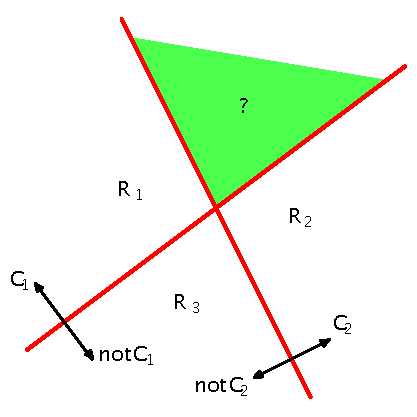
\includegraphics[width=\textwidth]{img/Bishop2006aa-p182-ch4-fig4-1-a.pdf}
%         \caption{One-Vs-Rest classification scheme}
%         \label{fig:Bishop2006aa-p182-ch4-fig4-1-a}
%     \end{subfigure}
%     ~ %add desired spacing between images, e. g. ~, \quad, \qquad, \hfill etc.
%       %(or a blank line to force the subfigure onto a new line)
%     \begin{subfigure}[b]{0.4\textwidth}
%         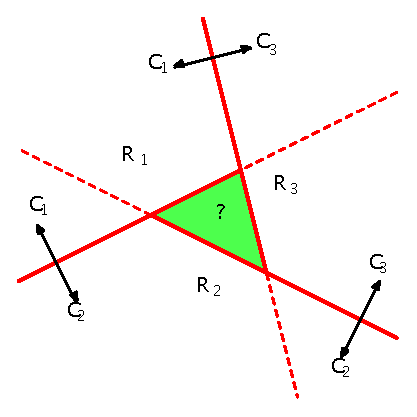
\includegraphics[width=\textwidth]{img/Bishop2006aa-p182-ch4-fig4-1-b.pdf}
%         \caption{One-Vs-One classification scheme}
%         \label{fig:Bishop2006aa-p182-ch4-fig4-1-b}
%     \end{subfigure}
%     \caption{: Ambiguous regions in the hypothesis space (\cite{Bishop:2006aa} Chapter 4, Figure 4.1) }
%     \label{fig:Bishop2006aa-p182-ch4-fig4-1}
% \end{figure}

\subsubsection{Generalized Linear Models}
\label{subs:Generalized Linear Models}


\subsubsection{Baysian Classifiers}
\label{subs:Probabilistic Classifiers}

\subsubsection{Decision Trees}
\label{subs:Decision Trees}

\subsubsection{Example-Based Classifiers}
\label{subs:Example-Based Classifiers}

\subsubsection{Ensemble Methods}
\label{subs:Ensemble Methods}

\subsubsection{Support Vector Machines}
\label{subs:Support Vector Machines}

\subsubsection{Neural Networks}
\label{subs:Neural Networks}

\subsection{Sequential Text Classification}
\label{sub:Sequential Text Classification}

\cite{Gers:1999aa} - Learning to forget: continual prediction with LSTM.

\subsection{Evaluation}
\label{sub:Evaluation}

In this section the basics of evaluating classification models for the given problem will be laid out. First the different evaluation schemes and their advantages or disadvantages are explained in the dichotomous case where only one class is to be predicted in terms of being active or not. Then these are generalized to the multi-label case where $K$ mutually exclusive classes are given. The last section extends this concept again towards so-called multi-label multi-output classification where several output labels can be predicted at the same time.

\subsubsection{Binary Classification}
\label{subs:Binary Classification}

In the binary case of classification we are given a single class $k$ and a set of labelled data points $\mathcal{D} = \{ (x_1, y_1), (x_2, y_2), \ldots, (x_n, y_n) \}$ where targets $y_i \in \{0, 1\}$ encode whether a data point $x_i$ belongs the class $c$ or not. The task is then to achieve correct classification of new data points without knowing the true label via a model function or predictor $f(\cdot)$.

To evaluate such a predictor it is useful to present the results in form of a contingency table as shown in table Table~\ref{table:contingency-table-2}, because it gives valuable insights about the performance of the prediction. The table shows the proportion of data points that belong to the class (RP) or not (RN) and were predicted correctly (TP) or incorrectly (FN), as well as the number of data samples that do not belong to the class (RN) and were falsely predicted to be in the class (FP) or correctly predicted to not be in the class (TN), and the same proportions for the positively (PP) and negatively (PN) predicted cases with respect to the true assignments to the data. N refers to the total amount of data points.

\begin{table}[h]
  \begin{center}
    \begin{tabular}{r | c c }
      & Real Positives (RP) & Real Negatives (RN) \\
      \hline
      Predicted Positives (PP) & True Positives (TP) & False Positives (FP) \\
      Predicted Negatives (PN) & False Negatives (FN) & True Negatives (TN) \\
    \end{tabular}
  \caption{Contingency table for binary classification}
  \label{table:contingency-table-2}
  \end{center}
\end{table}

\paragraph{Accuracy}
\label{par:Accuracy}

An intuitive choice towards classification is to simply ask which data points were correctly classified to belong to the class or not. In terms of the contingency table above the ratio of $(\text{TP} + \text{FP}) / (\text{N})$, commonly referred to as the ``accuracy'' of the classifier.

This choice can give a good intuition and it does capture the effectiveness on both true positives as well as true negatives, but it is strongly influenced by bias of the true and predicted class distribution (known as prevalence RP/N and label bias) as pointed out by~\cite{Powers:2011aa}. For example given a population of 900 positive and 100 negative examples, a predictor that simply always chooses a positive assignment can achieve accuracy of 90\% while it obviously is not a great predictor.

\textquote{There is a good reason why accuracy is not an appropriate measure for information retrieval problems. In almost all circumstances, the data is ex- tremely skewed: normally over 99.9\% of the documents are in the nonrele- vant category. A system tuned to maximize accuracy can appear to perform well by simply deeming all documents nonrelevant to all queries. Even if the system is quite good, trying to label some documents as relevant will almost always lead to a high rate of false positives. However, labeling all documents as nonrelevant is completely unsatisfying to an information retrieval system user. }\cite[Chapter 8.3, p.~155]{Manning:2008aa}

\paragraph{Precision, Recall and F1 Score}
\label{par:Precision, Recall and F1 Score}

In the field of Information Retrieval it is common practice to measure the effectiveness of a predictive system in terms of its precision and recall.
The precision of such system is \textquote{the proportion of retrieved material that is actually relevant} whereas the recall measures \textquote{proportion of relevant material actually retrieved in answer to a search request}~\cite{Rijsbergen:1979aa}. Formally these two measures are defined as:

\begin{equation}
    \text{Precision} = \frac{\text{TP}}{\text{TP} + \text{FP}}
\end{equation}
\begin{equation}
    \text{Recall} = \frac{\text{TP}}{\text{TP} + \text{FN}}
\end{equation}


As both, high precision and recall, are important for an robust information retrieval system they are typically combined into a single measure such as the F-measure, also referred to as F-score. The F-score is the weighted harmonic mean between precision and recall, derived from the measure of effectiveness proposed in~\cite{Rijsbergen:1979aa}. The most common form is the $F_1$ score  where precision and recall are assigned equal weight:
\begin{equation}
  \label{f1measure}
  F_1 = 2 \cdot \frac{\text{Precision} \cdot \text{Recall}}{\text{Precision} + \text{Recall}}
\end{equation}

The $F_1$ score has the advantage of its intuitive interpretability as both precision and recall are well understood measures and, analogous to recall, precision and accuracy, as it lives in the range $[0,1]$, giving a single number that can express the effectiveness of the system in terms of percentage.

The F1 score is widely used in the field of Machine Learning and Data Mining and thus it is an important measure to consider to compare results to outcomes of prior publications by others.
It is however important to point out that any version of the F-measure is a biased score as it \textquote{ignores TN which can vary freely without affecting the statistic}~\cite{Powers:2011aa}. This can affect the evaluation of a classifier when the class distribution is skewed (prevalence) or the classifier develops a bias towards certain classes (label bias), motivating the use of unbiased measures in these cases, such as the ones described next.

\paragraph{Informedness, Markedness and Matthews Correlation Coefficient}
\label{par:Informedness, Markedness and Matthews Correlation Coefficient}

\cite{Powers:2011aa} introduces unbiased analogue measures to Recall and Precision, called ``Informedness'' and ``Markedness'' respectively. As~\cite{Powers:2011aa} lays out, \blockquote{Informedness quantifies how informed a predictor is for the specified condition, and specifies the probability that a prediction is informed in relation to the condition (versus chance).}:

\begin{equation}
  \begin{split}
  \text{Informedness} &= \text{Recall} + \text{Inverse Recall} \text{ – } 1 \\
  &= 1 - \text{Miss Rate} - \text{Fallout} \\
  &= 1 - \frac{\text{FN}}{ \text{RN}} - \frac{\text{FP}}{\text{RP}}
  \end{split}
\end{equation}

Further he defines:
\blockquote{Markedness quantifies how marked a condition is for the specified predictor, and specifies the probability that a condition is marked by the predictor (versus chance).}

\begin{equation}
  \begin{split}
  \text{Informedness} &= \text{Recall} + \text{Inverse Recall} \text{ – } 1 \\
  &= 1 - \text{Miss Rate} - \text{Fallout} \\
  &= 1 - \frac{\text{FN}}{ \text{RN}} - \frac{\text{FP}}{\text{RP}}
  \end{split}
\end{equation}

Based on Informedness and Markedness we can then see that \emph{Matthews Correlation Coefficient} $r_{G}$, first proposed by~\cite{Matthews:1975aa}, is a score that balances these two measures:

\begin{equation}
  \begin{split}
  r_{G} &= \pm \sqrt{\text{Informedness} \cdot \text{Markedness}} \\
  &= \frac{(\text{TP} \cdot \text{TN} - \text{FP} \cdot \text{FN})}{(\text{TP} + \text{FN})(\text{FP} + \text{TN})(\text{TP} + \text{FP})(\text{FN} + \text{TN})}
\end{split}
\end{equation}

Matthews Correlation Coefficient can thus be used as unbiased alternative to the F-measure and offers a similar ease of interpretability as it ranges from -1 to 1, the former indicating a negative correlation or adverse estimation and the latter  indicating a perfect prediction, while a coefficient of 0 reflects chance.

\paragraph{Cross-Entropy}
\label{par:Cross-Entropy}

Another common way to evaluate classifiers is the \emph{cross-entropy} loss function:

\begin{equation}
  \mathbb{H}(p,q) = - \sum_n^N p_n \log q_n
\end{equation}

where $p$ and $q$ are discrete probability distributions. The \emph{cross-entropy} can be derived from the \emph{KL-divergence} as in~\cite[Chapter 2.8.2, p.~57]{Murphy:2012aa}:

\begin{equation}
  \begin{split}
  \mathbb{KL}(p,q) &= \sum_n^N p_n \log \frac{p_n}{q_n} \\
  &= \sum_n^N p_n \log p_n - \sum_n^N p_n \log q_n \\
  &= - \mathbb{H}(p) + \mathbb{H}(p,q)
\end{split}
\end{equation}

where $\mathbb{H}(p)$ is the regular entropy, i.e.\ the lower bound on the number of bits needed to transmit the state of a random variable (as in~\cite{Shannon:2001aa}), and $\mathbb{H}(p,q)$ is the cross-entropy, i.e. \textquote{the average number of bits needed to encode data coming from a source distribution $p$ when we use model $q$ to define our codebook}~\cite[Chapter 2.8.2, p.~57]{Murphy:2012aa}.

In the case of binary classification we can rewrite the cross-entropy into the following error or loss function of the learned weight vector:

\begin{equation}
  E(\mathbf{w}) =  -\log p(\mathbf{T} \mid \mathbf{w}) = - \sum_{n=1}^N {t_n \log y_n + (1 - t_n) \log (1 - y_n)}
\end{equation}

where $y_n$ denotes $y(x_n, \mathbf{w})$, the predicted output for datapoint $x_n$, $t_n$ denotes the $n$-th true label and $\mathbf{w}$ denotes the trained weight vector of the model, as in~\cite[Chapter 4.3.2, p.~205 ]{Bishop:2006aa}. This form is also known as the \emph{log loss} and it is commonly used with generalized linear models and neural networks (see e.g.~\cite[Chapter 4.3.2, p.~205 ]{Bishop:2006aa} and~\cite[Chapter 10.7, p.~251 ]{Alpaydin:2014aa}).

Thus, cross-entropy is a measure which is well-motivated from a information-theoretic perspective. On the downside it does not have an upper bound which makes it hard to interpret, as compared other scores that fall into [0, 1] or similar intervals.

\subsubsection{Multi-class Classification}
\label{subs:Multi-class Classification}

Multi-class classification refers to a generalization of the binary case where we aim to predict for each datapoint $x_i$ one of $K$ labels for the classes at hand. The target space $\mathcal{Y}$ can be represented with each $y_i \in \{ 0,1 \}^k$, known as \emph{one-hot encoding}, where each target is $c$-dimensional vector. Alternatively we can encode the targets as categorical variables $y_i \in {c_1, c_2, \ldots, c_k}$. The contingency table from the binary case can be extended as in table~\ref{table:contingency-table-k}, which is then commonly known as \emph{Confusion Matrix} or \emph{Error Matrix} \todo{citation for Confusion Matrix?}.

\begin{center}
  \begin{table}[h]
  \begin{tabular}{r | c c c c }
    & Real Class 1 & Real Class 2 & \ldots & Real Class $k$ \\
    \hline
    Predicted Class 1    & \ldots & \ldots & & \ldots \\
    Predicted Class 2    & \ldots & \ldots & & \ldots \\
    \ldots               & & & & \\
    Predicted Class $k$  & \ldots & \ldots & & \ldots \\
  \end{tabular}
  \caption{Contingency table for $k$ classes, also referred to as Confusion Matrix}
\label{table:contingency-table-k}
\end{table}
\end{center}

\paragraph{Averaging for Multi-class Recall, Precision and F1-Score}
\label{par:Averaging for Multi-class Recall, Precision and F1-Score}

By definition, Recall, Precision and thus also the F-measure are defined for the dichotomous classification case, however they can be extended towards multiple classes by averaging. Two common methods are described in~\cite[Chapter 13.6, p.~280]{Manning:2008aa}: \textquote{Macroaveraging computes a simple average over classes. Microaveraging pools per-document decisions across classes, and then computes an effectiveness measure on the pooled contingency table.}
It is important to note that \textquote{macroaveraging gives equal weight to each class, whereas microaveraging gives equal weight to each per-document classification decision. Because the F1 measure ignores true negatives and its magnitude is mostly determined by the number of true positives, large classes dominate small classes in microaveraging.}~\cite[Chapter 13.6, p.~280]{Manning:2008aa}. Formally these averaging schemes can be defined as follows, with R denoting the Recall and P the Precision.

\begin{equation}
  \text{R}_{\text{micro}} = \frac{\sum_{k=1}^K \text{TP}_k }{ \sum_{k=1}^K \text{TP}_k + \text{FN}_k } \qquad
  \text{R}_{\text{macro}} = \frac{\sum_{k=1}^K \text{R}_k }{ K }
\end{equation}
\begin{equation}
  \text{P}_{\text{micro}} = \frac{\sum_{k=1}^K \text{TP}_k }{ \sum_{k=1}^K \text{TP}_k + \text{FP}_k } \qquad
  \text{P}_{\text{macro}} = \frac{\sum_{k=1}^K \text{P}_k }{ K }
\end{equation}

And respectively:

\begin{equation}
  \text{F}_{1 \text{micro}} = 2 \cdot \frac{\text{P}_{\text{micro}} \cdot \text{R}_{\text{micro}} }{\text{P}_{\text{micro}} + \text{R}_{\text{micro}} } \qquad
  \text{F}_{1 \text{macro}} = 2 \cdot \frac{\text{P}_{\text{macro}} \cdot \text{R}_{\text{macro}} }{\text{P}_{\text{macro}} + \text{R}_{\text{macro}} }
\end{equation}

\paragraph{Matthews Correlation Coefficient for K classes}
\label{par:Matthews Correlation Coefficient for K classes}

\cite{Gorodkin:2004aa} introduced a way to extend Matthews Correlation Coefficient to the multi-class case using a generalization of Pearson’s Correlation Coefficient. The coefficient is then defined as:

\begin{equation}
  R_k  = \frac{\text{COV}(X, Y)}{\sqrt{\text{COV}(X, X) \ \text{COV}(Y, Y)}}
\end{equation}

Where $\text{COV}$ is the covariance function:

\begin{align}
  \text{COV}(X, Y) &= \sum_{k=1}^K w_k \text{COV}(X_k, Y_k) \\
  &= \frac{1}{K} \sum_{n=1}^N \sum_{k=1}^K (X_{nk} - \overline{X_k})(Y_{nk} - \overline{Y_k})
\end{align}

Similar extensions have been proposed, such as the Confusion Entropy (CEN) as described in~\cite{Jurman:2012aa}. The article concludes:

\blockquote{Confusion Entropy [\ldots] is probably the finest measure and it shows an extremely high level of discriminancy even between very similar confusion matrices. However, this feature is not always welcomed, because it makes the interpre- tation of its value quite harder, expecially when considering sit- uations that are naturally very similar (e.g, all the cases with MCC=0). Moreover, CEN may show erratic behaviour in the binary case.

In this spirit, the Matthews Correlation Coefficient is a good compromise between reaching a reasonable discriminancy degree among different cases, and the need for the practitioner of a easily interpretable value expressing the type of misclassification associated to the chosen classifier on the given task. We showed here that there is a strong linear relation between CEN and a logarithmic function of MCC regardless of the dimension of the considered problem. Furthermore, MCC behaviour is totally consistent also for the binary case.

This given, we can suggest MCC as the best off-the-shelf evaluating tool for general purpose tasks, while more subtle measures such as CEN should be reserved for specific topic where more refined discrimination is crucial.}

Thus Matthews Correlation Coefficient is the preferred measure when possible.

\paragraph{Categorical Cross-Entropy}
\label{par:Categorical Cross-Entropy}

The \emph{cross-entropy} loss function as defined above in Section~\ref{par:Cross-Entropy} extends to the multi-class case quite naturally:

\begin{equation}
  E(\mathbf{w}_1, \ldots, \mathbf{w}_k) = -\ln p(\mathbf{T} \mid \mathbf{w}_1, \ldots, \mathbf{w}_k) = - \sum_{n=1}^N \sum_{k=1}^K t_{nk} \ln y_{nk}
\end{equation}

where $y_{nk} = y_k (\phi_n)$, and $\mathbf{T}$ is an  $N \times K$ matrix of target variables with elements $t_{nk}$ (see as in~\cite[Chapter 4.3.4, p.~209 ]{Bishop:2006aa}). This form is also referred to as \emph{multi-class log loss} and gives an aggregated loss over all classes. \todo{more detail?}

\subsubsection{Multi-label Classification *}
\label{subs:Multi-label Classification}

\subsection{Visualization}

\subsubsection{PCA}
\label{sub:PCA}

\subsubsection{t-SNE}
\label{sub:t-SNE}

% !TEX root = ../thesis.tex
% !TEX spellcheck = en-US

%% In a thesis, every section starts a new page, hence \clearpage
\clearpage

\section{Exploration}
\label{sec:Exploration}

\subsection{Project Brief}
\label{sub:Project Brief}

The objective of this thesis was to find interesting and novel ways to use the various data that get generated through Sanoma's  recruitment platform \emph{Oikotie Työpaikat}. This was stated in the research plan as follows:

\blockquote{Find an application of data mining / machine learning to the customer-generated data on the recruitment platform Oikotie Työpaikat which has the potential of bringing value to the user of the platform and is technically feasible in the scope of a master’s thesis. Further define and investigate a research problem that is essential to this application by researching literature and previous work on similar problems trying different approaches based on the literature using the results and learnings to create an improved approach.}



% - brief
% - given data
% - interest?
% - approach
% - found problem: predicting audience and popularity of job ads
% - in order to do so: learn about structure of job ads
% - problem setting as supervised task,
% - get data by free collection:
%   - to predict paragraphs
%   - to learn about how humans interpret and carry out this task
% - experiments: grouping tags automatically vs manually
% - predicting with tf.idf
% - reading up on how to write good job ads
% - can be grouped into 6 categories
% - framed as new mulit-class problem and setting up data collection
% - results: distribution and statistics, most of the data can somewhat go into these categories (other is the smallest amount)
% - then trying to evaluate the best method or combination of methods



\subsection{Approach}
\label{sub:Approach}

\subsection{Understanding structure of job ads}
\label{sub:Understanding structure of job ads}
% 
% # personnel selection
% \cite{Chien:2008aa} - improving personnel selection with data mining
% \cite{Saidi-Mehrabad:2007aa} - The development of an expert system for effective selection and appointment of the jobs applicants in human resource management.
% \cite{Hokey-Min:2003aa} - Developing the profiles of truck drivers for their successful recruitment and retention: A data mining approach.
% \cite{Youyou:2015aa} - Computer-based personality judgments are more accurate than those made by humans
%
% # careers
% \cite{Shahaf:2012aa} - metro maps of science
%
% # formal vs informal language
% \cite{Faruqui:2011aa} - I Thou Thee, Thou Traitor": Predicting Formal vs. Informal Address in English Literature.
% \cite{Brooke:2014aa} -  Computational Approaches to Style and the Lexicon
%
% \cite{Lee:2015:RJO:2700171.2791048} - On Recommending Job Openings
%
% \cite{Luhn:1958aa} - A Business Intelligence System


\subsection{Crowdsourced Data Collection (*)}

\todo{Describe data format}

In order to perform supervised learning labelled data was needed for training. Together with the process of reframing of the research problem this was approached in an iterative way. First a quick prototypical tool was built to collect labels in a crowd-sourced fashion. This allowed getting more knowledge about the problem itself, especially with regards to how humans perform the task of labelling topics of text sections, and to perform first experiments of algorithmically achieving meaningful results in agreement to human behavior on this task.
Then these learnings were taken into consideration when re-scoping the research problem and according to that data was collected using the micro tasking service CrowdFlower\footnote{\textquote{CrowdFlower is a data enrichment, data mining and crowdsourcing company [\ldots]. The company's software as a service platform allows users to access an online workforce of millions of people to clean, label and enrich data.} Source: \url{https://en.wikipedia.org/wiki/CrowdFlower}, Company website: \url{https://www.crowdflower.com}}, leading to a quality dataset of labelled sentences from job ads.

\subsubsection{Explorative Paragraph Dataset}

\todo{Picture of software setup?}

To collect first data a tool was build, consisting of a Node.js\footnote{[\ldots] Node.js is an open-source, cross-platform runtime environment for developing server-side Web applications. \url{https://nodejs.org/}} server using MongoDB\footnote{\textquote{MongoDB is a free and open-source cross-platform document-oriented database [\ldots].} Source: \url{https://en.wikipedia.org/wiki/Node.js}, Website: \url{https://www.mongodb.com}} as a database and communicating via a JSON with a simple website front-end using the mustache template engine\footnote{\textquote{Mustache is a simple web template system.} Source: \url{https://en.wikipedia.org/wiki/Mustache_(template_system)}, Website: \url{https://mustache.github.io}}.
The tool is online\footnote{\url{http://thesis.cwestrup.de/jobad-tagger/}} and it's source code is publicly available on GitHub\footnote{\url{https://github.com/cle-ment/thesis-tagger}} with it's API documentation hosted online as well\footnote{\url{http://thesis.cwestrup.de/jobad-tagger/apidoc/}}.

The data generated by using the free-form text description of each job ad and splitting it into paragraphs as can be seen in the software package as well\footnote{\url{https://github.com/cle-ment/thesis-tagger/blob/master/pre-processing.ipynb}}.

The goal of this prototype tool for data collection was on the one hand to acquire data in order to carry our first experiments as fast as possible, and on the other hand to gain a deeper understanding about the research problem itself by giving an open, unbiased task to the participants. In particular the question at hand was how humans label the content of the different parts of a job ad.

The exact task given to the participants was ``Describe what each section is about by adding one or more tags/keywords to it''. They were shown a job ad that was split into paragraphs and besides each paragraph was a text field to enter 1 or more tags.

\begin{figure}[h]
  \centering
  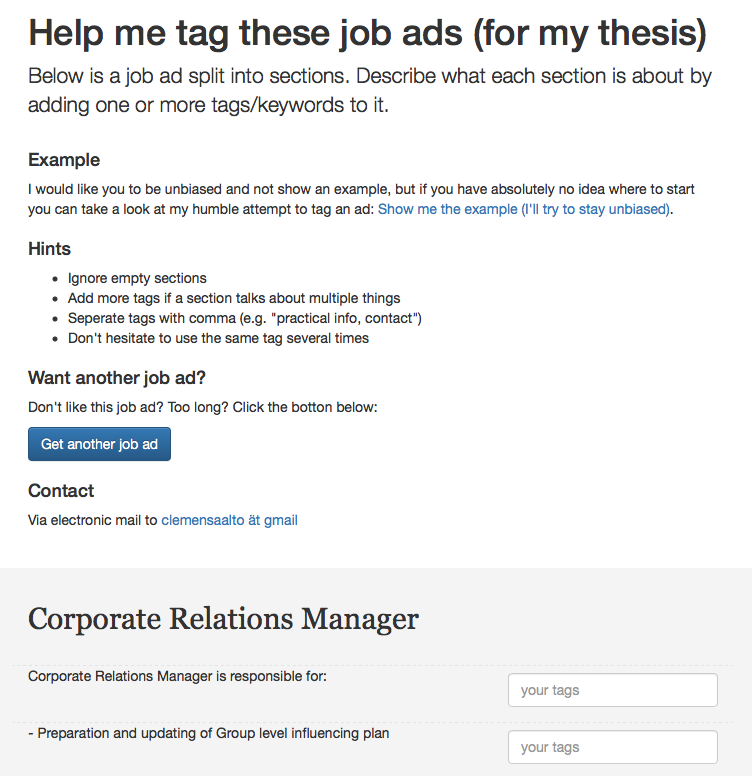
\includegraphics[width=\textwidth]{img/thesis-tagger-interface.png}
  \caption{Screen capture of the interface of the tagging tool}
\label{fig:thesis-tagger-interface}
\end{figure}

In a first step the tool was only shown to 3 participants to get immediate feedback if the user interface had flaws and whether the task was understood.   Based on this feedback the tool was improved by providing an example for the participants and then tested with a slightly larger group of 12 persons. After correcting a few minor details in the user interface a public link was then shared via social media and other channels with as many people as possible. A few days later the tool was then also shared internally within Sanoma where it was set up as a competition to tag the most possible job ads.

In total 91 job ads were tagged, resulting in 379 tagged text sections and 358 tags.

\todo{Describe data: Different characteristics}
\todo{show distribution?}
\todo{show embedding visualizations}

\begin{figure}[h]
    \centering
    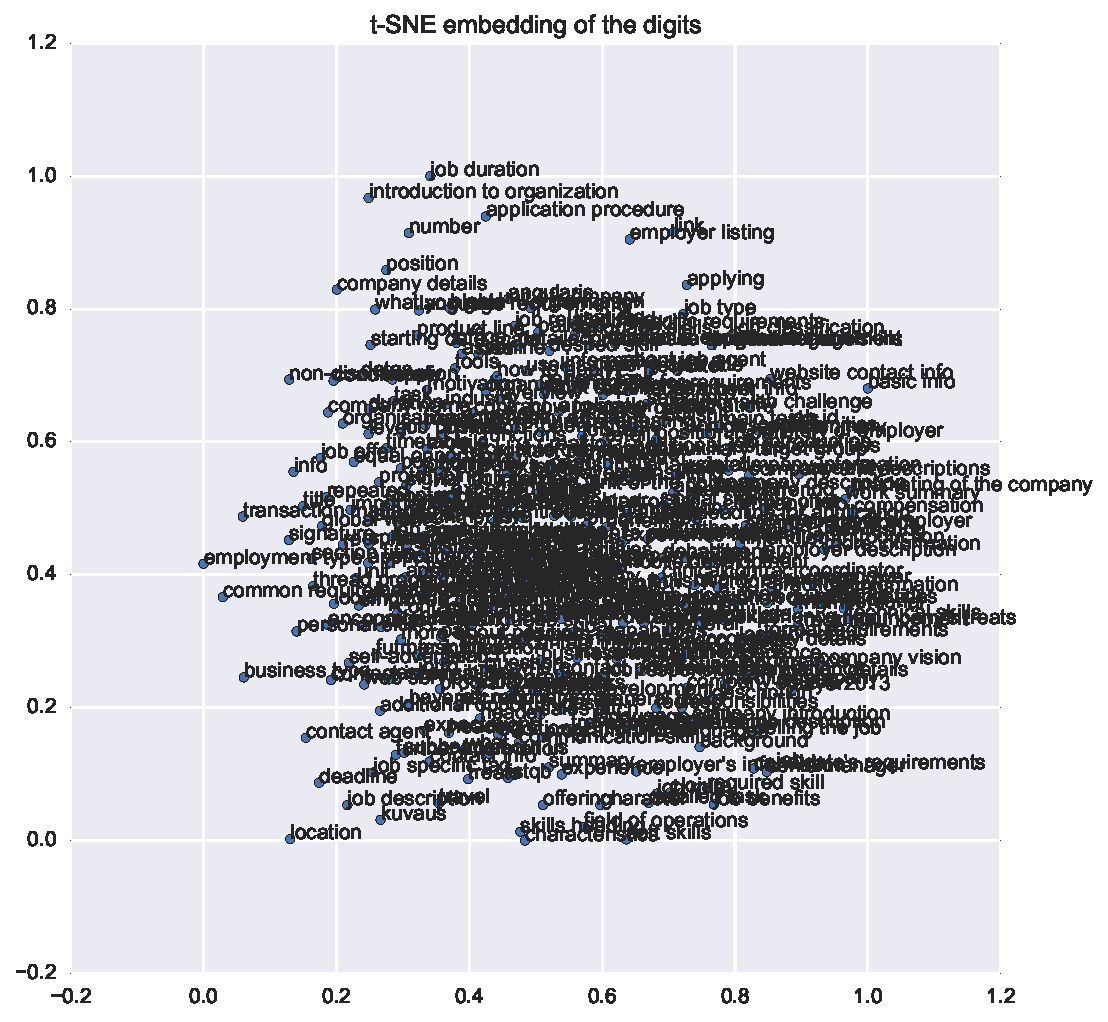
\includegraphics[width=\textwidth]{img/paragraph-data-tSNE.pdf}
    \caption{t-SNE Embedding}
\label{fig:paragraph-data-tSNE}
\end{figure}

\begin{figure}[h]
    \centering
    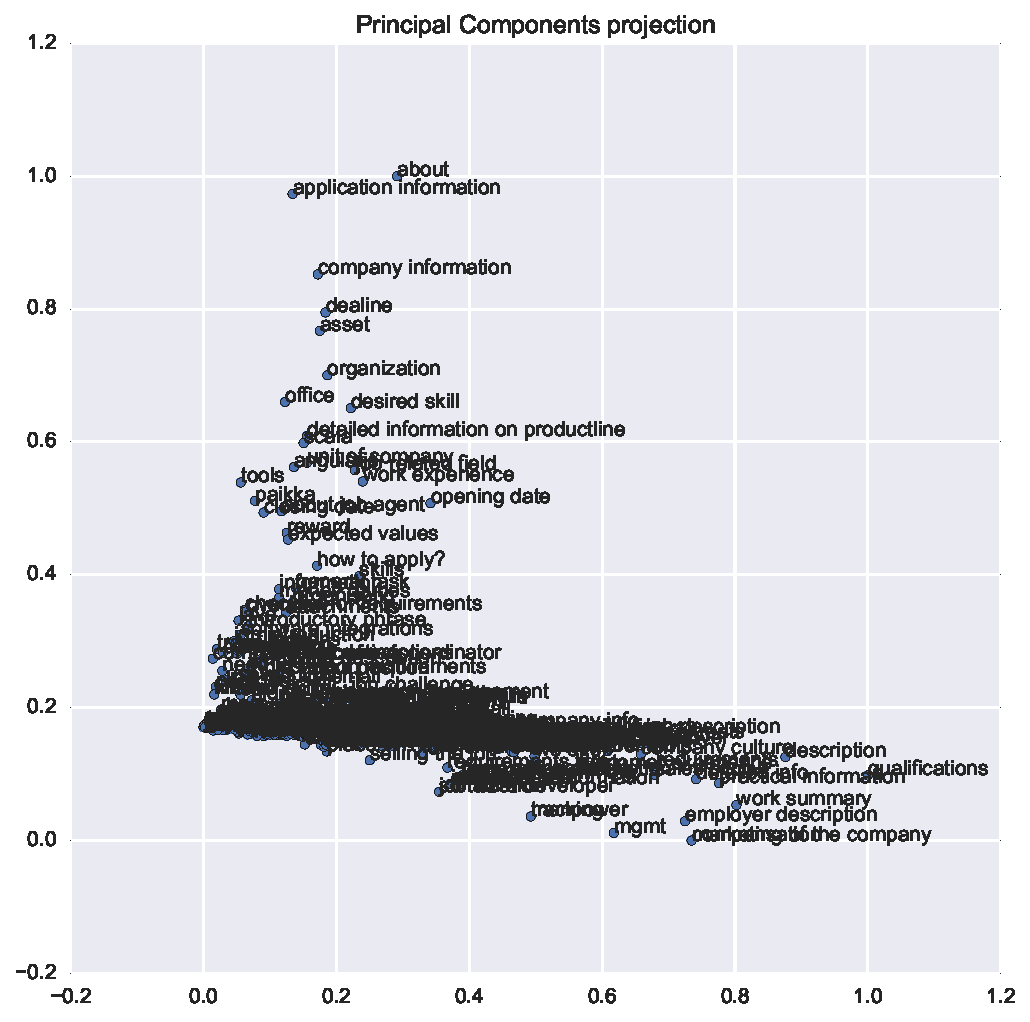
\includegraphics[width=\textwidth]{img/paragraph-data-principal-components-projection.pdf}
    \caption{Principal Components Projection}
\label{fig:paragraph-data-principal-components-projection}
\end{figure}

\todo{Comparison one-vs-rest and one-vs-one against linear machine}
\todo{Visualizations and embeddings of data in 2D (and decision boundaries?)}
\todo{show T-SNE embeddings of doc2vec vectors}

% !TEX root = ../thesis.tex
% !TEX spellcheck = en-US


\clearpage

\section{Methods}
\label{sec:Methods}

% How did I approach the problem, what methods did I evaluate

\clearpage

\section{Experimental Evaluation}
\label{sec:Experimental Evaluation of Multi-class Prediction of Semantic Categories for Text in Job Advertisements}

\subsection{Problem definition}

\subsection{Evaluation of Vector Space Models}

\subsubsection{Experimental Setup}
\label{subs:Experimental Setup}

\todo{Doc2Vec model is evaluated in 2 ways (normal and trained on inferred vectors)}

\todo{say why using the sentence dataset here}
\todo{reference jupyter notebook here}
% http://localhost:8888/notebooks/thesis/experiments/vector-space-models/Vector%20Space%20Models.ipynb#Setup

As Section~\ref{sec:vector-space-models} explains, a popular way to approach text classification and other tasks in natural language processing is to build a language model by creating explicit representations of the objects or entities to be processed in a vector space. Such vectors can be used as features for a learning algorithm. Depending on the representation they can also carry further meaning, such as to encode notions of similarity of associativity between the objects.

In order to determine effective vector space representations for the task of sentence classification, a set of experiments was carried out to study and compare different approaches. Each method was studied with regards to the effect of its hyper-parameters on effectiveness when producing an input space to different classifiers, but also time and memory requirements at training and inference time are taken into account \todo{actually discuss time and memory requirements}.

In order to compare the effectiveness for the sentence classification task as discussed in Section\todo{reference section here} each labelled document was transformed into a vector space representation using the different methods and then used for classification with a simple logistic regression classifier (\todo{link to logistic regression classifier explanation here}). Performance was then compared with regards to Matthews Correlation Coefficient for K classes (Section~\ref{par:Matthews Correlation Coefficient for K classes}) and the Accuracy \todo{link accuracy?} of the classifier.

\subsubsection{Baselines Classifiers: Uniform and Stratified Guessing}
\label{subs:baselines-classifiers}

As a baseline for comparing the performance of classification two different guessing strategies were used, namely uniform and stratified guessing.
Uniform guessing refers to a predictor that samples from the given classes assuming a uniform distribution whereas stratified guessing takes the label distribution in the data as the underlying probability distribution.
Then both methods just sample from these distributions to produce ``predictions'', while ignoring the actual input data. Both, uniform and stratified guessing achieve a Matthews Correlation Coefficient score of around 0 (averaged over 1000 runs) as expected for guessing strategies (see Section~\ref{subs:informedness-markedness-mcc}). On the other hand the accuracy for uniform guessing is around 0.16 which corresponds to $1/\text{K}$ for the K classes and around 0.26 for stratified guessing which reflects the skew of the label distribution.
Figure~\ref{fig:exp-vector-space-conf-matrix-guessing} shows the confusion matrices for these baseline variants in absolute and normalized form, revealing the properties of these guessing strategies.

\begin{figure}[h]
 % From http://localhost:8888/notebooks/thesis/experiments/vector-space-models/Vector%20Space%20Models.ipynb#Baseline:-Guessing-Strategies
    \centering
    \begin{subfigure}[b]{0.47\textwidth}
        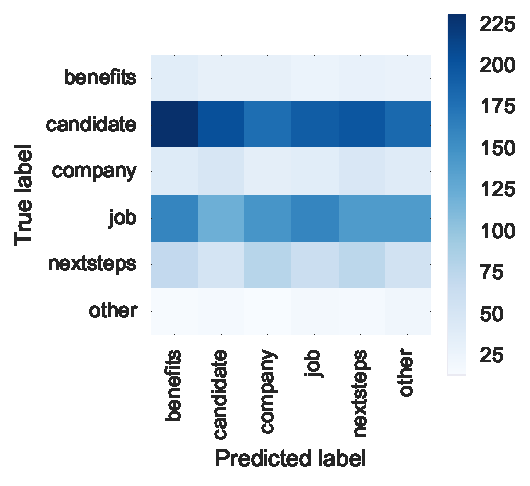
\includegraphics[width=\textwidth]{img/exp-vector-space-conf-matrix-guessing-uniform.pdf}
        \caption{Uniform, absolute}
\label{fig:exp-vector-space-conf-matrix-guessing-uniform}
    \end{subfigure}
~
    %add desired spacing between images, e. g. ~, \quad, \qquad, \hfill etc.
    %(or a blank line to force the subfigure onto a new line)
    \begin{subfigure}[b]{0.48\textwidth}
        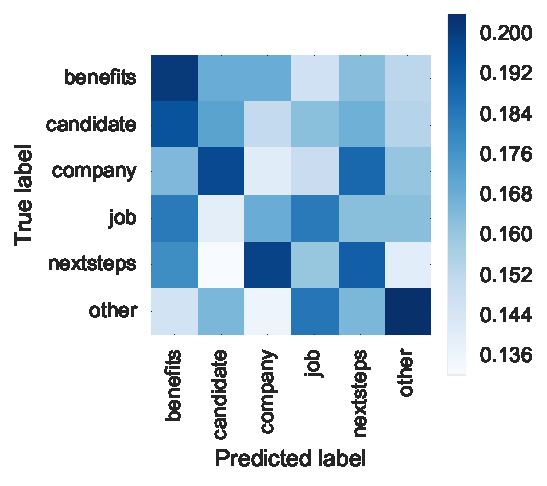
\includegraphics[width=\textwidth]{img/exp-vector-space-conf-matrix-guessing-uniform-normalized.pdf}
        \caption{Uniform, normalized}
\label{fig:exp-vector-space-conf-matrix-guessing-uniform-normalized}
    \end{subfigure}
~
    \begin{subfigure}[b]{0.47\textwidth}
        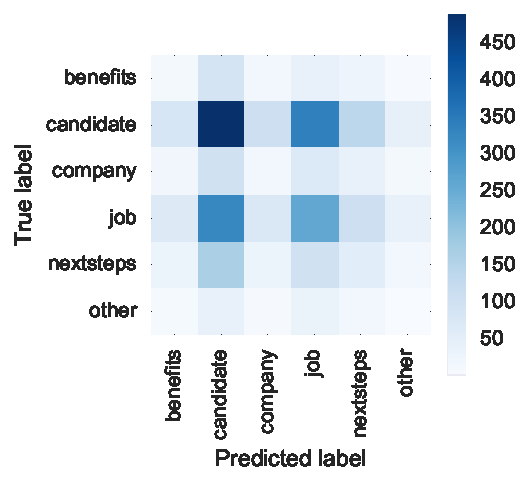
\includegraphics[width=\textwidth]{img/exp-vector-space-conf-matrix-guessing-stratified.pdf}
        \caption{Stratified, absolute}
\label{fig:exp-vector-space-conf-matrix-guessing-stratified}
    \end{subfigure}
~
    %add desired spacing between images, e. g. ~, \quad, \qquad, \hfill etc.
    %(or a blank line to force the subfigure onto a new line)
    \begin{subfigure}[b]{0.48\textwidth}
        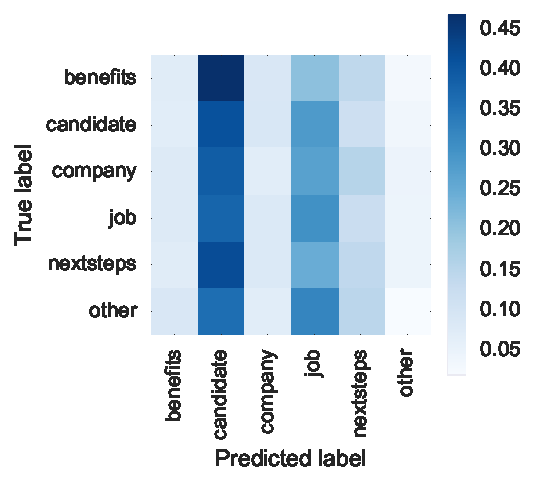
\includegraphics[width=\textwidth]{img/exp-vector-space-conf-matrix-guessing-stratified-normalized.pdf}
        \caption{Stratified, normalized}
\label{fig:exp-vector-space-conf-matrix-guessing-stratified-normalized}
    \end{subfigure}
    \caption{Confusion matrices of uniform and stratified guessing strategies. }
\label{fig:exp-vector-space-conf-matrix-guessing}
\end{figure}

\subsubsection{N-gram Language Models}

The first class of language models that was investigated for the task of multi-class classification are N-gram models that were explained in Section~\ref{subs:n-gram-language-models}. As mentioned, in essence this type of model relies on simple statistics which makes for straightforward computation but at the same time comes at cost of expressiveness, especially in terms of temporal dependencies between words.

As N-grams models come in a variety of variants the most important ones were used as hyper-parameters to the model and a grid search was carried out over a wide range of combinations over these. The specific hyper-parameter settings are listed in Table~\ref{tab:ngram-parameters}. The grid search was optimized with regards to \emph{Matthews Correlation Coefficient} (see Section~\ref{par:Matthews Correlation Coefficient for K classes}) using 5-fold cross-validated with three standard classifiers: Logistic Regression and Naive Bayes and SVM.

\begin{table}[h]
  \begin{center}
  \begin{tabular}{ l l l}
    \toprule
    Hyper-Parameter & N-gram Type: Words & N-gram Type: Characters \\
    \midrule
    N-gram Range (Range) & [1,1], [1,2], [1,3], [2,3], [3,3] & [1,5], [1,10], [5,10], [5,15] \\
    Stop Words & English, None & N/A \\
    Vector Size (Size) & 10, 100, 300 & 10, 100, 300 \\
    IDF & Yes, No & Yes, No \\
    Norm & L1, L2, None & L1, L2, None \\
    Sub-linear TF & Yes, No & Yes, No \\
    \bottomrule
  \end{tabular}
  \caption{Parameter search space word and character level N-gram models}
\label{tab:Ngram Parameters}
\end{center}
\end{table}

The 5 best results of these exhaustive grid searches can be seen in Table~\ref{tab:Ngram Grid Search} below.

\begin{table}[h]
  \begin{center}
  \begin{tabular}{ l l l l l l l l }
    \toprule
    Type & Range & Stop words & Size & IDF & Norm & Sub-linear TF & MCC Score \\
    \midrule
    Word & [1,1] & None & 300 & Yes &  & Yes & 0.689 \\
    Word & [1,1] & None & 300 & Yes &  & No & 0.687 \\
    Word & [1,1] & None & 300 & No &  & Yes & 0.682 \\
    Word & [1,1] & None & 300 & No &  & No & 0.682 \\
    Word & [1,1] & None & 300 & Yes & L2 & Yes & 0.68 \\
    % Word & [1,1] & None & 300 & Yes & L2 & No & 0.678 \\
    % Word & [1,2] & None & 300 & No &  & Yes & 0.677 \\
    % Word & [1,2] & None & 300 & Yes & L2 & Yes & 0.676 \\
    % Word & [1,2] & None & 300 & Yes & L2 & No & 0.675 \\
    % Word & [1,2] & None & 300 & No &  & No & 0.675 \\
    \midrule
    Word & [1,1] & None & 300 & No & & Yes & 0.659  \\
    Word & [1,1] & None & 300 & No & & No & 0.656 \\
    Word & [1,2] & None & 300 & No & & Yes & 0.655 \\
    Word & [1,2] & None & 300 & No & & No & 0.655 \\
    Word & [1,3] & None & 300 & No & & No & 0.65 \\
    % Word & [1,1] & None & 300 & Yes & L2 & Yes & 0.648 \\
    % Word & [1,1] & None & 300 & Yes & L2 & No & 0.648 \\
    % Word & [1,3] & None & 300 & No & & Yes & 0.648 \\
    % Word & [1,2] & None & 300 & Yes & L2 & No & 0.647 \\
    % Word & [1,2] & None & 300 & Yes & L2 & Yes & 0.646 \\
    \midrule
    Word & [1,1] & None & 300 & Yes & & Yes & 0.689 \\
    Word & [1,1] & None & 300 & Yes & & No  & 0.689 \\
    Word & [1,2] & None & 300 & Yes & & Yes & 0.677 \\
    Word & [1,2] & None & 300 & Yes & & No  & 0.677 \\
    Word & [1,3] & None & 300 & Yes & & Yes & 0.674 \\
    % Word & [1,3] & None    & 300 & Yes & & No  & 0.673 \\
    % Word & [1,1] & English & 300 & Yes & & Yes & 0.65 \\
    % Word & [1,1] & English & 300 & Yes & & No  & 0.65 \\
    % Word & [1,2] & English & 300 & Yes & & No  & 0.649 \\
    % Word & [1,2] & English & 300 & Yes & & Yes & 0.648 \\
    \bottomrule
  \end{tabular}
  \caption{Top 5 results of grid search over hyper-parameter space as listed in Table~\ref{tab:Ngram Parameters} using 5-fold cross-validated Logistic Regression (top), Naive Bayes (middle) and SVM (bottom) classifiers.}
\label{tab:Ngram Grid Search}
\end{center}
\end{table}

\todo{Why are the grid scores lower than the latter scores on the train/test split? Because they're averaged and only on the training data?}

Across all classifiers the following results on the hyper-parameters can be observed:

\paragraph{Type}
\label{par:Type}
Words as the atomic unit for N-grams consistently lead to better results. This is understandable as the search space of combinations of characters is significantly larger than the search space of known words.

\paragraph{Range}
\label{par:Range}
There are slight differences to be observed between the three classifiers used, but with all three models the best performance is achieved using Unigrams. Also all of the top results across all classifiers include Unigrams in the model while extending the range towards bigrams or trigrams.

\paragraph{Stop Words}
\label{par:Stop Words}
None of the top results of the performed grid searches used stop words. This is interesting as using stop-words to remove hand-picked, highly frequent words that do not carry much meaning is common practice. It seems there is information carried within these stop words. Of course this outcome is also influenced by the particular stop-list used (see Section~\ref{subp:Stop words}).

\paragraph{Size (matters)}
\label{par:Size}
For the searched settings the largest vector dimensionality of 300 achieves the best performance. This is not surprising as higher-dimensional vectors can capture more information about N-gram occurrences. However in practice the vector size must be limited as it grows with the vocabulary --- potentially at an exponential rate if N-grams other than Unigrams are used. Also very high dimensionality often leads to decreased performance in terms of generalization of the model.

\paragraph{IDF}
\label{par:IDF}
There is no consensus between the classifiers on whether or not to weigh the N-gram frequencies by the \emph{inverse document frequency} (see Section~\ref{subp:TF.IDF weighting}). Thus it seems advisable to lead this parameter free for and evaluate both variants with a given classifier. For logistic regression however the performance differences are marginal and so the choice for this parameter seems somewhat arbitrary.

\paragraph{Norm}
\label{par:Norm}
Is seems that normalizing the vectors in most cases does not lead to any performance gains. Again this is an often recommended practice but here it does not seem to add any value to the model.


\paragraph{Sub-linear TF}
\label{par:Sub-linear TF}
Applying sub-linear TF (see Section~\ref{subp:Sublinear TF scaling}) does not seem to affect the results much and the choice of this parameter can hence be chosen almost arbitrarily as well, although here for all three classifiers applying it leads to a marginal improvement.

Table~\ref{tab:Ngram Grid Search Scores} shows the scores of each classifier using the best N-gram model. It is evident that here logistic regression actually performs best as it offers both, a good accuracy as well as the highest score for Matthews Correlation Coefficient.

\begin{table}[h]
  \begin{center}
  \begin{tabular}{ r | *2l | *2l }
    \toprule
     & \multicolumn{2}{c|}{Training} & \multicolumn{2}{|c}{Validation}\\
    Classifier & Accuracy & MCC & Accuracy & MCC \\
    \midrule
    Logistic Regression & 0.824 & 0.761 & 0.787 & 0.708 \\
    Naive Bayes         & 0.769 & 0.681 & 0.767 & 0.677 \\
    SVM                 & 0.835 & 0.681 & 0.786 & 0.700 \\
    \bottomrule
  \end{tabular}
  \caption{Performance of each best N-gram model with Logistic Regression and Naive Bayes on the validation data}
\label{tab:Ngram Grid Search Scores}
\end{center}
\end{table}

\begin{figure}[h]
    \centering
    \begin{subfigure}[b]{0.32\textwidth}
        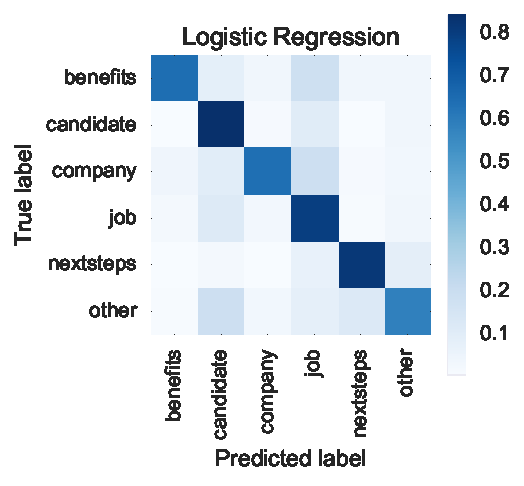
\includegraphics[width=\textwidth]{img/exp-vector-space-conf-matrix-ngram-logreg-normalized.pdf}
        \caption{Logistic Regression}
\label{fig:exp-vector-space-conf-matrix-ngram-logreg-normalized}
    \end{subfigure}
    \begin{subfigure}[b]{0.32\textwidth}
        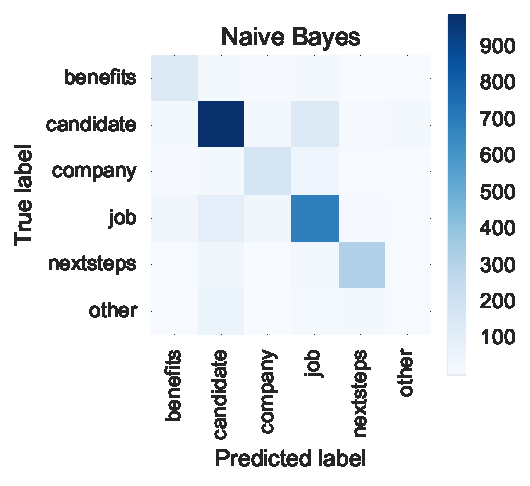
\includegraphics[width=\textwidth]{img/exp-vector-space-conf-matrix-ngram-naivebayes-normalized.pdf}
        \caption{Naive Bayes}
\label{fig:exp-vector-space-conf-matrix-ngram-naivebayes-normalized}
    \end{subfigure}
    \begin{subfigure}[b]{0.32\textwidth}
        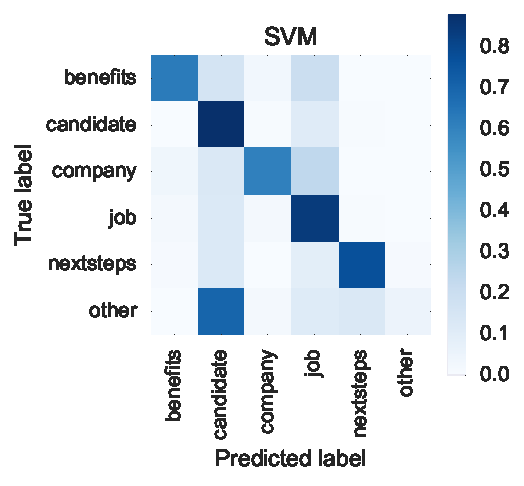
\includegraphics[width=\textwidth]{img/exp-vector-space-conf-matrix-ngram-svm-normalized.pdf}
        \caption{SVM}
\label{fig:exp-vector-space-conf-matrix-ngram-svm-normalized}
    \end{subfigure}
    \caption{Normalized confusion matrices all three classifiers using the best N-gram model found via cross-validated grid search. Both Naive Bayes as well as SVM show label bias towards the prevalent class \emph{candidate}.}
\label{fig:exp-vector-space-conf-matrix-ngram}
\end{figure}
\todo{properly align visualization}

Figure~\ref{fig:exp-vector-space-ngram} shows projections of the of the constructed feature space using the best model that was optimized with Logistic Regression. This visualization shows the separability of the classes in this space. Especially the PCA projection here reveals that it is clearly possible to separate the classes until a certain point.

\begin{figure}[h]
    \centering
    \begin{subfigure}[b]{0.48\textwidth}
      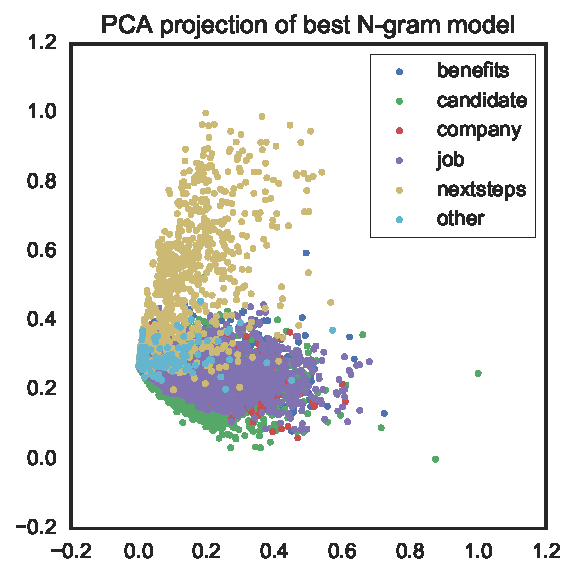
\includegraphics[width=\textwidth]{img/exp-vector-space-ngram-pca.pdf}
      \caption{PCA projection}
\label{fig:exp-vector-space-ngram-pca}
    \end{subfigure}
~
    %add desired spacing between images, e. g. ~, \quad, \qquad, \hfill etc.
    %(or a blank line to force the subfigure onto a new line)
    \begin{subfigure}[b]{0.48\textwidth}
      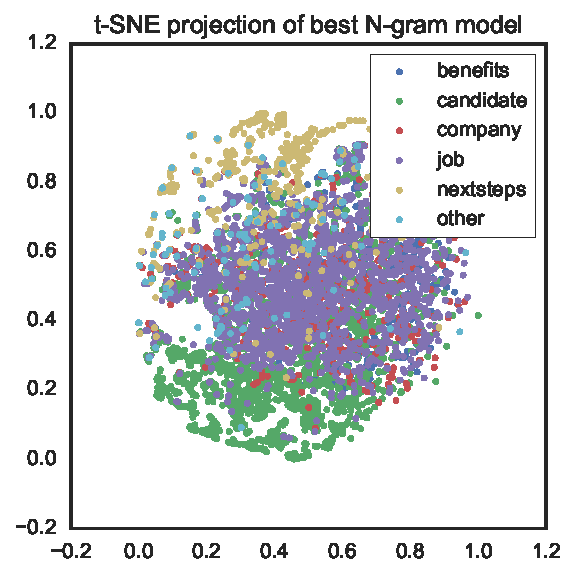
\includegraphics[width=\textwidth]{img/exp-vector-space-ngram-tsne.pdf}
      \caption{t-SNE projection}
\label{fig:exp-vector-space-ngram-tsne}
    \end{subfigure}
    \caption{Document vectors produced by the best N-gram model (optimized w.r.t. Logistic Regression) projected onto the first 2 principal components (left) and project using t-SNE projection.}
\label{fig:exp-vector-space-ngram}
\end{figure}

\subsubsection{Bag-of-Means --- An Averaged Word2Vec Model}

Next a Bag-of-Means model as described in Section~\ref{subp:Bag-of-Means} was evaluated with the same set of classifiers. The model was evaluated on the same test and training data split as used for the N-gram model above. As a basis the pre-trained word-vectors from the Google News dataset\footnote{The dataset contains contains 300-dimensional vectors for 3 million words and phrases. The phrases were obtained using a simple data-driven approach described in~\cite{Mikolov:2013ab}. The dataset can be obtained on the following website: \url{https://code.google.com/archive/p/word2vec/}} were used and then for each document all word vectors were average to obtain the document vector. The results can be seen in Table~\ref{tab:Bag-Of-Means Results}.

\begin{table}[h]
  \begin{center}
  \begin{tabular}{ r | *2l | *2l }
    \toprule
     & \multicolumn{2}{c|}{Training} & \multicolumn{2}{|c}{Validation}\\
    Classifier & Accuracy & MCC & Accuracy & MCC \\
    \midrule
    Logistic Regression & 0.797 & 0.722 & 0.784 & 0.702 \\
    Naive Bayes         & 0.337 & 0.271 & 0.320 & 0.251 \\
    SVM                 & 0.545 & 0.356 & 0.562 & 0.379 \\
    \bottomrule
  \end{tabular}
  \caption{Performance base classifiers using the Bag-of-Means model}
\label{tab:Bag-Of-Means Results}
\end{center}
\end{table}

The model performs well using Logistic Regression and is almost on par with the best N-gram model. This is surprising as performance previously reported to be rather poor as mention in Section~\ref{subp:Bag-of-Means}. On the other hand the variance in results between the classifiers is huge and especially Naive Bayes seems to perform extremely poor. Further investigation into the use of different classifiers could shed light into these diverging results which are not observed using the N-gram models in the section above. The confusion matrices in Figure~\ref{fig:exp-vector-space-conf-matrix-bom} reveal strong label bias in the case of Naive Bayes and SVM, although it is unclear where this stems from. Figure~\ref{fig:exp-vector-space-bom} makes clear though that there is a somewhat meaningful mapping into the feature space. \todo{mention one-vs-all scheme for log reg? also for ngrams above}

\begin{figure}[h]
    \centering
    \begin{subfigure}[b]{0.32\textwidth}
        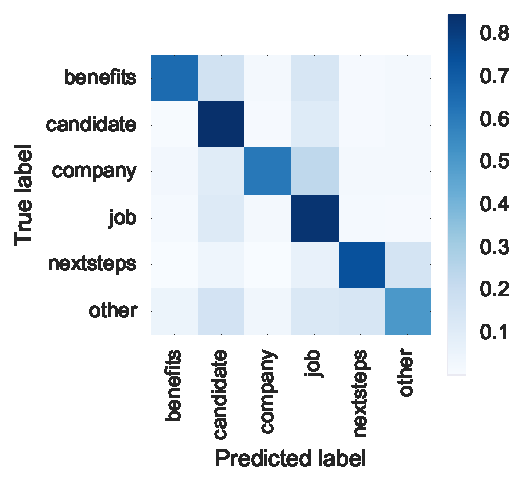
\includegraphics[width=\textwidth]{img/exp-vector-space-conf-matrix-bom-logreg-normalized.pdf}
        \caption{Logistic Regression}
\label{fig:exp-vector-space-conf-matrix-bom-logreg-normalized}
    \end{subfigure}
    \begin{subfigure}[b]{0.32\textwidth}
        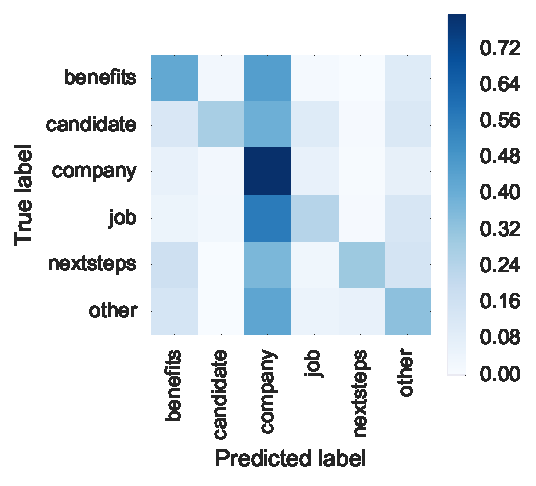
\includegraphics[width=\textwidth]{img/exp-vector-space-conf-matrix-bom-naivebayes-normalized.pdf}
        \caption{Naive Bayes}
\label{fig:exp-vector-space-conf-matrix-bom-naivebayes-normalized}
    \end{subfigure}
    \begin{subfigure}[b]{0.32\textwidth}
        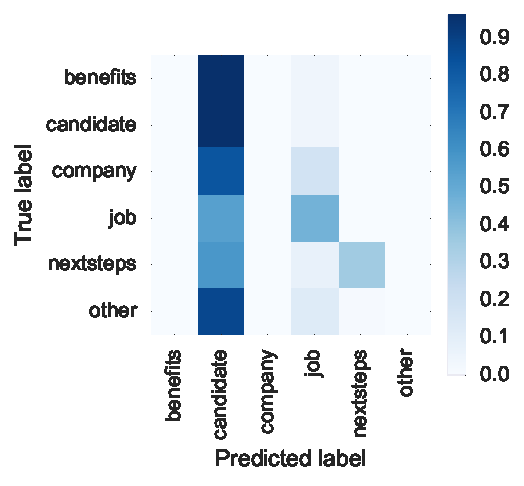
\includegraphics[width=\textwidth]{img/exp-vector-space-conf-matrix-bom-svm-normalized.pdf}
        \caption{SVM}
\label{fig:exp-vector-space-conf-matrix-bom-svm-normalized}
    \end{subfigure}
    \caption{Normalized confusion matrices of all three classifiers using the Bag-of-Means model.}
\label{fig:exp-vector-space-conf-matrix-bom}
\end{figure}

\begin{figure}[h]
    \centering
    \begin{subfigure}[b]{0.48\textwidth}
      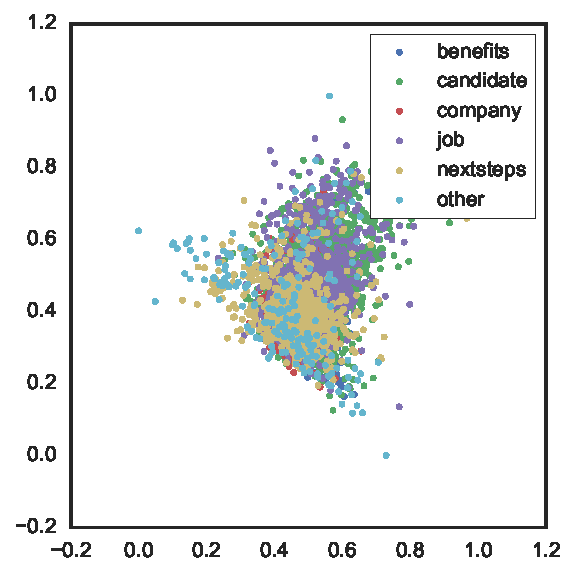
\includegraphics[width=\textwidth]{img/exp-vector-space-bom-pca.pdf}
      \caption{PCA projection}
\label{fig:exp-vector-space-bom-pca}
    \end{subfigure}
~
    %add desired spacing between images, e. g. ~, \quad, \qquad, \hfill etc.
    %(or a blank line to force the subfigure onto a new line)
    \begin{subfigure}[b]{0.48\textwidth}
      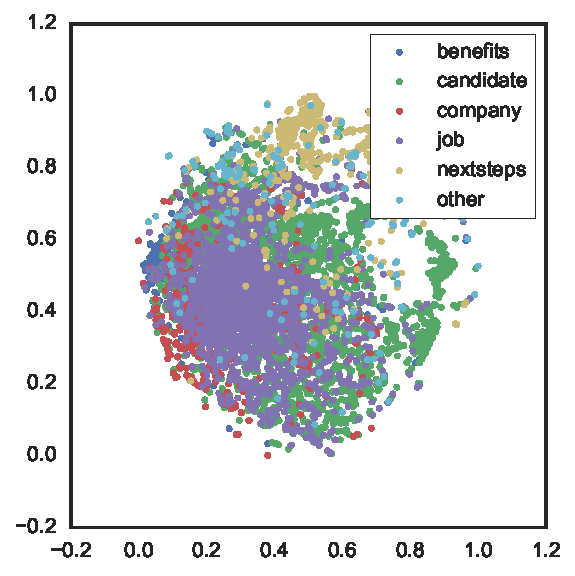
\includegraphics[width=\textwidth]{img/exp-vector-space-bom-tsne.pdf}
      \caption{t-SNE projection}
\label{fig:exp-vector-space-bom-tsne}
    \end{subfigure}
    \caption{Document vectors produced by Bag-of-Means model (optimized w.r.t. Logistic Regression) projected onto the first 2 principal components (left) and projected using t-SNE projection. It is clear that even though the vectors are simply obtained by averaging they do indeed produce somewhat seperable manifolds.}
\label{fig:exp-vector-space-bom}
\end{figure}

\subsubsection{Paragraph Vectors using Distributed Representations}

Next a vector space model was build using the approach proposed by~\cite{Le:2014aa} and described in more detail in Section~\ref{par:Distributed representations for documents}. Again there are several hyper-parameters to this model that are described in Section~\ref{subs:Language Models using Distributed Representations} and turn out to have a huge influence on its performance as the results below indicate. As this model is computationally quite expensive a grid search as for the N-gram model above was infeasible. Thus the effect of the hyper-parameters was studied by just varying them one at a time while keeping the others fixed, using a Logistic Regression classifier with 5-fold cross-validation.
The next sections will briefly outline the results of these tests:\footnote{All tables in this section will use the following abbreviations: \emph{type}: Model Type, i.e. PV-DM vs. PV-DBOW; \emph{size}: Vector Size; \emph{window}: Window Size; \emph{negative}: Negative Sampling value $k$; \emph{hs}: Hierarchical Softmax used; \emph{sample}: Frequent word sub-sampling threshold; \emph{MCC}: Matthews Correlation Coefficient}

\paragraph{Vector Size}
As was to expect the vector size of the model correlates with the performance. Again the highest chosen dimensionality was 300 which yielded the best results with a Matthews Correlation Coefficient of 0.53, however the difference to a 100-dimensional model was marginal with 1\% absolute improvement. Surprisingly even a 10-dimensional vector space model is capable of achieving almost best results with a difference of only 2\% to the 300-dimensional model. Even a 2-dimensional model could achieve a MCC score of 14\%.

\begin{table}[h]
  \begin{center}
    \begin{tabular}{ c | *2c | *2c }
      \toprule
       & \multicolumn{2}{c|}{MCC Training} & \multicolumn{2}{|c}{MCC Test}\\
      Vector Size & Trained & Inferred & Trained & Inferred \\
      \midrule
      2 & 0.324 & 0.265 & 0.189 & 0.257 \\
      10 & 0.467 & 0.411 & 0.319 & \textbf{0.404} \\
      100 & 0.510 & 0.399 & 0.357 & 0.400 \\
      300 & 0.572 & 0.362 & 0.344 & 0.398 \\
      \bottomrule
    \end{tabular}
  \caption{Matthews Correlation Coefficient with varying vector size.}
\label{tab:Paragraph Vector Parameter Results Size}
\end{center}
% Previous results:
% PV-DM & 2   & 10 & 3 & 1 & 0 & 0.536 \\
% PV-DM & 10  & 10 & 3 & 1 & 0 & 0.522 \\
% PV-DM & 100 & 10 & 3 & 1 & 0 & 0.514 \\
% PV-DM & 300 & 10 & 3 & 1 & 0 & 0.144 \\
\end{table}

\paragraph{Frequent Word Sub-Sampling}
Frequent word sub-sampling can boost performance quite much, but again choosing the right value for this hyper-parameter is key. The training behavior with different sampling thresholds differs quite much. Figure~\ref{fig:exp-vector-space-doc2vec-param-sample} shows the training with different values with 100 passes over the dataset. A good value seems to be $10^{-5}$ which achieves an MCC score of 0.697 and is on-par with the best N-gram model. Interestingly not using sub-sampling in this setup seemed to be overfitting as the score decreases quite drastically with more training passes. A similar effect is observed with a higher threshold of $10^{-4}$ but much less strong. Choosing a lower threshold of $10^{-6}$ leads to very poor performance with an MCC score of only 0.07.

\begin{table}[h]
  \begin{center}
    \begin{tabular}{ c | *2c | *2c }
      \toprule
       & \multicolumn{2}{c|}{MCC Training} & \multicolumn{2}{|c}{MCC Test}\\
      Sub-sampling threshold & Trained & Inferred & Trained & Inferred \\
      \midrule
      No sub-sampling & 0.531 & 0.364 & 0.340 & 0.380 \\
      1e-4 & 0.628 & 0.372 & 0.3151 & \textbf{0.401} \\
      1e-5 & 0.608 & 0.248 & 0.180 & 0.250 \\
      1e-6 & 0.583 & 0.156 & 0.107 & 0.128 \\
    \bottomrule
  \end{tabular}
  \caption{Matthews Correlation Coefficient with varying frequent word sub-sampling threshold.}
\label{tab:Paragraph Vector Parameter Results Sample}
\end{center}
% Previous results:
% PV-DM & 300 & 10 & 3 & 1 & 0 & 0.244 \\
% PV-DM & 300 & 10 & 3 & 1 & 1e-4 & 0.556 \\
% PV-DM & 300 & 10 & 3 & 1 & 1e-5 & 0.698 \\
% PV-DM & 300 & 10 & 3 & 1 & 1e-6 & 0.071 \\
\end{table}


\begin{figure}[h]
    \centering
    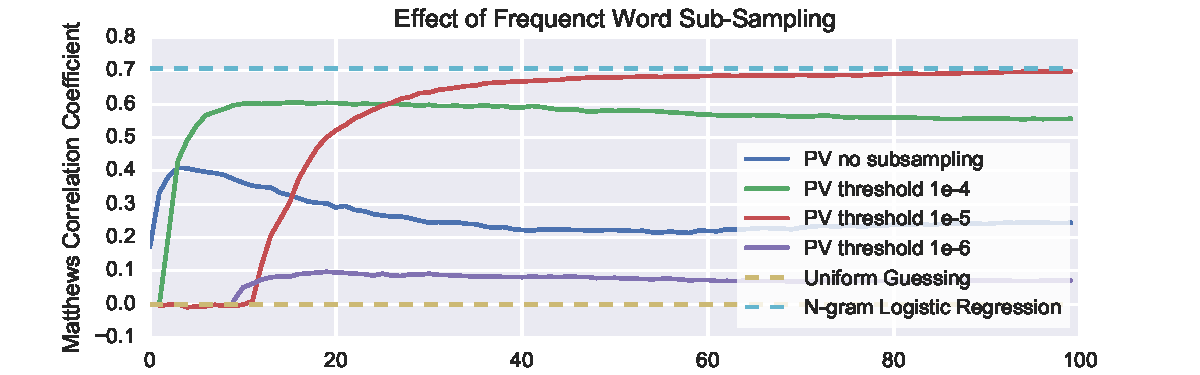
\includegraphics[width=\textwidth]{img/exp-vector-space-doc2vec-param-sample.pdf}
    \caption{Training of document vectors with different sub-sampling thresholds.}
  \label{fig:exp-vector-space-doc2vec-param-sample}
\end{figure}

\paragraph{Hierarchical Softmax}
Using hierarchical softmax increased the performance, leading to a 12\% absolute difference in terms of MCC score. This result is counter-intuitive as using the hierarchical softmax should as an approximation be less performant. However it might simply mitigate overfitting of the model.

\begin{table}[h]
  \begin{center}
    \begin{tabular}{ c | *2c | *2c }
      \toprule
       & \multicolumn{2}{c|}{MCC Training} & \multicolumn{2}{|c}{MCC Test}\\
      Hierarchical Softmax & Trained & Inferred & Trained & Inferred \\
      \midrule
      Used & 0.374 & 0.279 & 0.202 & 0.299 \\
      Not used & 0.519 & 0.404 & 0.366 & \textbf{0.408} \\
    \bottomrule
  \end{tabular}
  \caption{Matthews Correlation Coefficient with and without using hierarchical softmax.}
\label{tab:Paragraph Vector Parameter Results Hierarchical Softmax}
\end{center}
% Previous results:
% PV-DM & 100 & 10 & 3 & 0 & 0 & 0.398 \\
% PV-DM & 100 & 10 & 3 & 1 & 0 & 0.520 \\
\end{table}

\paragraph{Negative Sampling}
Negative Sampling generally increased the performance of the model and smaller values actually worked best out of the tested settings from 0 to 6. Choosing the number of negative samples to be 2 resulted in the best performance, but the absolute difference in performance was only about 6\% of achieved MMC score.

\begin{table}[h]
  \begin{center}
    \begin{tabular}{ c | *2c | *2c }
      \toprule
       & \multicolumn{2}{c|}{MCC Training} & \multicolumn{2}{|c}{MCC Test}\\
      Negative Sampling Value & Trained & Inferred & Trained & Inferred \\
      \midrule
      0 & 0.422 & 0.322 & 0.251 & 0.310 \\
      2 & 0.565 & 0.367 & 0.342 & 0.395 \\
      4 & 0.470 & 0.386 & 0.348 & \textbf{0.398} \\
      6 & 0.481 & 0.340 & 0.320 & 0.360 \\
    \bottomrule
  \end{tabular}
  \caption{Matthews Correlation Coefficient with varying negative sampling value.}
\label{tab:Paragraph Vector Parameter Results Negative Sampling}
\end{center}
% Previous results:
% PV-DM & 100 & 10 & 0 & 1 & 0 & 0.530 \\
% PV-DM & 100 & 10 & 1 & 1 & 0 & 0.541 \\
% PV-DM & 100 & 10 & 2 & 1 & 0 & 0.536 \\
% PV-DM & 100 & 10 & 3 & 1 & 0 & 0.524 \\
% PV-DM & 100 & 10 & 4 & 1 & 0 & 0.516 \\
% PV-DM & 100 & 10 & 5 & 1 & 0 & 0.498 \\
% PV-DM & 100 & 10 & 6 & 1 & 0 & 0.482 \\
\end{table}

\paragraph{Window Size}
Window sizes of 5, 10 and 15 were experimented with which increase or decrease the width of context the model is trained on. Here a window size of 10 showed best results. It is safe to assume that increasing the window size much further does not lead to any improvement in the model as the correlation with the word should become weaker the farther we move away from it in a document or text.


\begin{table}[h]
  \begin{center}
    \begin{tabular}{ c | *2c | *2c }
      \toprule
       & \multicolumn{2}{c|}{MCC Training} & \multicolumn{2}{|c}{MCC Test}\\
      Window size & Trained & Inferred & Trained & Inferred \\
      \midrule
      5 & 0.537 & 0.363 & 0.375 & \textbf{0.412} \\
      10 & 0.523 & 0.363 & 0.402 & 0.404 \\
      15 & 0.518 & 0.359 & 0.390 & 0.405 \\
    \bottomrule
    \end{tabular}
  \caption{Matthews Correlation Coefficient with varying window size.}
\label{tab:Paragraph Vector Parameter Results Window Size}
\end{center}
% Previous results:
% PV-DM & 100 & 5 & 3 & 1 & 0 & 0.508 \\
% PV-DM & 100 & 10 & 3 & 1 & 0 & 0.523 \\
% PV-DM & 100 & 15 & 3 & 1 & 0 & 0.510 \\
\end{table}

\paragraph{PV-DBOW versus PM-DV}
Both models for paragraph vectors proposed in~\cite{Le:2014aa} were tried, namely Distributed Bag of Words version of Paragraph Vector (PV-DBOW) and Distributed Memory version of Paragraph Vec- tor (PV-DM). In these tests the DBOW model achieves significantly better results with an MCC that is 14\% than the PV-DM model in absolute terms. This is in contrast with the results in the aforementioned paper, where the authors state that \textquote{PV-DM is consistently better than PV-DBOW.}~\cite{Le:2014aa}.

\begin{table}[h]
  \begin{center}
    \begin{tabular}{ c | *2c | *2c }
      \toprule
       & \multicolumn{2}{c|}{MCC Training} & \multicolumn{2}{|c}{MCC Test}\\
      Window size & Trained & Inferred & Trained & Inferred \\
      \midrule
      PV-BBOW & 0.626 & 0.610 & 0.543 & \textbf{0.580} \\
      PV-DM & 0.519 & 0.405 & 0.366 & 0.411 \\
    \bottomrule
    \end{tabular}
    \caption{Matthews Correlation Coefficient using the two models proposed in~\cite{Le:2014aa}.}
\label{tab:Paragraph Vector Parameter Results PV-DBOW versus PM-DV}
\end{center}
% Previous results:
% PV-DM & 100 & 10 & 3 & 1 & 0 & 0.521 \\
% PV-BBOW & 100 & 10 & 3 & 1 & 0 & 0.667 \\
\end{table}

\paragraph{Evaluating the best hyper-parameter setting}

Taking the learnings about the effects of the different hyper-parameters to the performance of the model a subset of models were tested in search of the best hyper-parameter selection. The results of these experiments can be seen in Table~\ref{tab:Paragraph Vector Parameter Results Best}.

A few interesting observations can be made here. First, as indicated before, the model is highly sensitive to the settings of the hyper-parameters. Secondly we can see that the hyper-parameters interact quite strongly in some combinations. This leads to a different behavior in performance for some of the hyper-parameters than identified in the above sections, depending on what the other hyper-parameters settings are.

For instance using hierarchical softmax decreases performance when setting all other parameters to individually optimal settings, as opposed to in the previous experiment above.
\todo{write a bit more here}

\begin{table}[h]
  \begin{center}
  \begin{tabular}{ *6l | l }
    \toprule
    type & size & window & negative & hs & sample & MCC  \\
    \midrule
    PV-DM & 300 & 10 & 3 & 0 & 1e-5 & 0.707 \\
    PV-BBOW & 300 & 10 & 3 & 0 & 1e-5 & 0.724 \\
    PV-BBOW & 300 & 10 & 3 & 1 & 1e-5 & 0.665 \\
    \bottomrule
  \end{tabular}
  \caption{Matthews Correlation Coefficient of different models when trying to find the best hyper-parameter setting.}
\label{tab:Paragraph Vector Parameter Results Best}
\end{center}
\end{table}

\subsubsection{Paragraph Vectors using pre-initialized weights *}

In another experiment the weight matrix for the words was initialized with pre-trained weights from from the Google News dataset.

\subsubsection{Paragraph Vectors using context sentences *}

\todo{This section in further research? Because it would have to be done for N-grams as well (building a model with the context around a sentence) and it doesn't fit the task (only sentence given). Could also go into exploration}

\subsubsection{Inversion of Distributed Language Representations (??)}

\todo{if this is described here it has to go into background as well}

\subsubsection{Discussion *}


\subsubsection{Evaluation of Classification Algorithms for Vector Space Models *}

\paragraph{Logistic Regression *}

\paragraph{Decision Tree *}

\paragraph{Naive Bayes *}

\paragraph{SVM *}
\paragraph{KNN *}
\paragraph{Random Forest *}
\paragraph{Neural Networks *}
\paragraph{Convolutional Neural Networks *}

\paragraph{Discussion *}


\subsection{Evaluation of Sequential Text Classification *}


\subsubsection{Experimental Setup *}

\subsubsection{Character-based LSTM *}

\subsubsection{Character-based Multi-task LSTM *}

\subsubsection{Discussion *}

\subsection{Comparison}

% !TEX root = ../thesis.tex
% !TEX spellcheck = en-US

\clearpage
\section{Discussion and Conclusions}

\subsection{Discussion of Experimental Results}

\subsection{Conclusions}
\label{subs:conclusions}

\begin{itemize}
  \item As in many areas of machine learning much work has been going into feature engineering but it seems that feature learning, while much more computationally expensive, surpasses the potential of engineered feature representations. Deep learning and meta-learning are mature enough to make up for the gap that has been there for years: To achieve performance that is good enough to make an algorithmic system usable in production, huge amounts of research and engineering went into feature engineering and finally the performance of these methods can be matched and even surpassed by automated methods or learning features. (link here NG's transfer learning work, also Schmidhubers work of meta-learning and on function prediction etc)
  \item There is more need to understand the representations of such feature learning systems though, statistics are quite easy to understand but weights of a neural network don't tell much. There is however potential for learning ``better statistics'' ourselves, e.g. how to efficiently learn a language (by looking at explicit indermediate representations of the states of a NN)
  \item
\end{itemize}


\subsection{Contributions *}
\label{sub:contributions}

\begin{itemize}
  \item compare n-gram and doc2vec (?)
  \item
\end{itemize}

\subsection{Proposal for Future Research}
\label{sub:further-research}

Make this a structured prediction task: Closer to the original task of finding the semantic structure of a job ad. Predict a whole job, automatically chop it into categories. The knowledge about the context of the sentence carries strong prior knowledge for deciding a sentence category. Using hierarchical models or priors might make a big difference. Also in the sequential modeling setting this will most probably improve performance significantly.

\begin{itemize}
  \item how well do word2vec and comparable methods generalize: e.g.\ initialize a text corpus with word vectors from a bigger corpus (Google News), then train an RNN to predict the next word vector using the small corpus but use the bigger corpus to validate and see if words in bigger corpus can be inferred
  \item trajectory based algorithms (word trajectory through space for a sentence)
  \item Compare with standard benchmarks (TREC etc)
  \item Meta- / Transfer-learning: OCR with simultaneous LM learning (e.g. predict next character)
  \item Try on Finnish data !!!
  \item Try longer parts again maybe with better seperation (paragraphs). Doc2vec gets way better accuracy when documents are longer
  \item Doc2Vec, evaluate how close inferred vectors are to trained vectors
  \item combine sequential approaches with representations gained from external knowledge or trained simultaneously (learning embeddings for semantic concepts)
  \item for complex models like CNNs and RNNs need more data!
\end{itemize}


\paragraph{Trajectory -Based Algorithms on Text}
\label{par:Trajectory Algorithms on Text}
As shown in \cite{Mikolov:2013ac} and related work that was outlined in Section\todo{reference here} vector space models for text can capture very subtle semantic relationships between words by their location in the vector space. When


\subsection{Learnings}
\label{sub:learnings}

\begin{itemize}
  \item focusing on both, building a working system (engineering) and exploring new directions (science), is hard
  \item problem framing is hard
  \item Learned AWS
  \item building pipelines
  \item deep learning
  \item collecting data
\end{itemize}


%% Bibliography

\clearpage
%% The \phantomsection command is nessesary for hyperref to jump to the
%% correct page, in other words it puts a hyper marker on the page.
\phantomsection
\addcontentsline{toc}{section}{\refname}
%\addcontentsline{toc}{section}{References}
\bibliography{literature/thesis-research.bib}
\bibliographystyle{apalike}
%\nocite{*}

%% Appendix

% !TEX root = ../thesis.tex
% !TEX spellcheck = en-US

%% Equations, tables and figures have their own numbering in Appendices
\renewcommand{\theequation}{B\arabic{equation}}
\setcounter{equation}{0}
\renewcommand{\thefigure}{B\arabic{figure}}
\setcounter{figure}{0}
\renewcommand{\thetable}{B\arabic{table}}
\setcounter{table}{0}


%% Appendices
\clearpage

\thesisappendix

\section{Appendix \label{A}}

\todo{Add list of english stop words used for ngrams (sklearn list)}
\todo{Add first Ngram TF.IDF experiment}

\subsection{Stopwords for N-grams}
\label{sec:appendix-stopwords}

a
about
above
across
after
afterwards
again
against
all
almost
alone
along
already
also
although
always
am
among
amongst
amoungst
amount
an
and
another
any
anyhow
anyone
anything
anyway
anywhere
are
around
as
at
back
be
became
because
become
becomes
becoming
been
before
beforehand
behind
being
below
beside
besides
between
beyond
bill
both
bottom
but
by
call
can
cannot
cant
co
computer
con
could
couldnt
cry
de
describe
detail
do
done
down
due
during
each
eg
eight
either
eleven
else
elsewhere
empty
enough
etc
even
ever
every
everyone
everything
everywhere
except
few
fifteen
fify
fill
find
fire
first
five
for
former
formerly
forty
found
four
from
front
full
further
get
give
go
had
has
hasnt
have
he
hence
her
here
hereafter
hereby
herein
hereupon
hers
herself
him
himself
his
how
however
hundred
i
ie
if
in
inc
indeed
interest
into
is
it
its
itself
keep
last
latter
latterly
least
less
ltd
made
many
may
me
meanwhile
might
mill
mine
more
moreover
most
mostly
move
much
must
my
myself
name
namely
neither
never
nevertheless
next
nine
no
nobody
none
noone
nor
not
nothing
now
nowhere
of
off
often
on
once
one
only
onto
or
other
others
otherwise
our
ours
ourselves
out
over
own
part
per
perhaps
please
put
rather
re
same
see
seem
seemed
seeming
seems
serious
several
she
should
show
side
since
sincere
six
sixty
so
some
somehow
someone
something
sometime
sometimes
somewhere
still
such
system
take
ten
than
that
the
their
them
themselves
then
thence
there
thereafter
thereby
therefore
therein
thereupon
these
they
thick
thin
third
this
those
though
three
through
throughout
thru
thus
to
together
too
top
toward
towards
twelve
twenty
two
un
under
until
up
upon
us
very
via
was
we
well
were
what
whatever
when
whence
whenever
where
whereafter
whereas
whereby
wherein
whereupon
wherever
whether
which
while
whither
who
whoever
whole
whom
whose
why
will
with
within
without
would
yet
you
your
yours
yourself
yourselves

\clearpage
\section{Appendix \label{B}: Experiments}

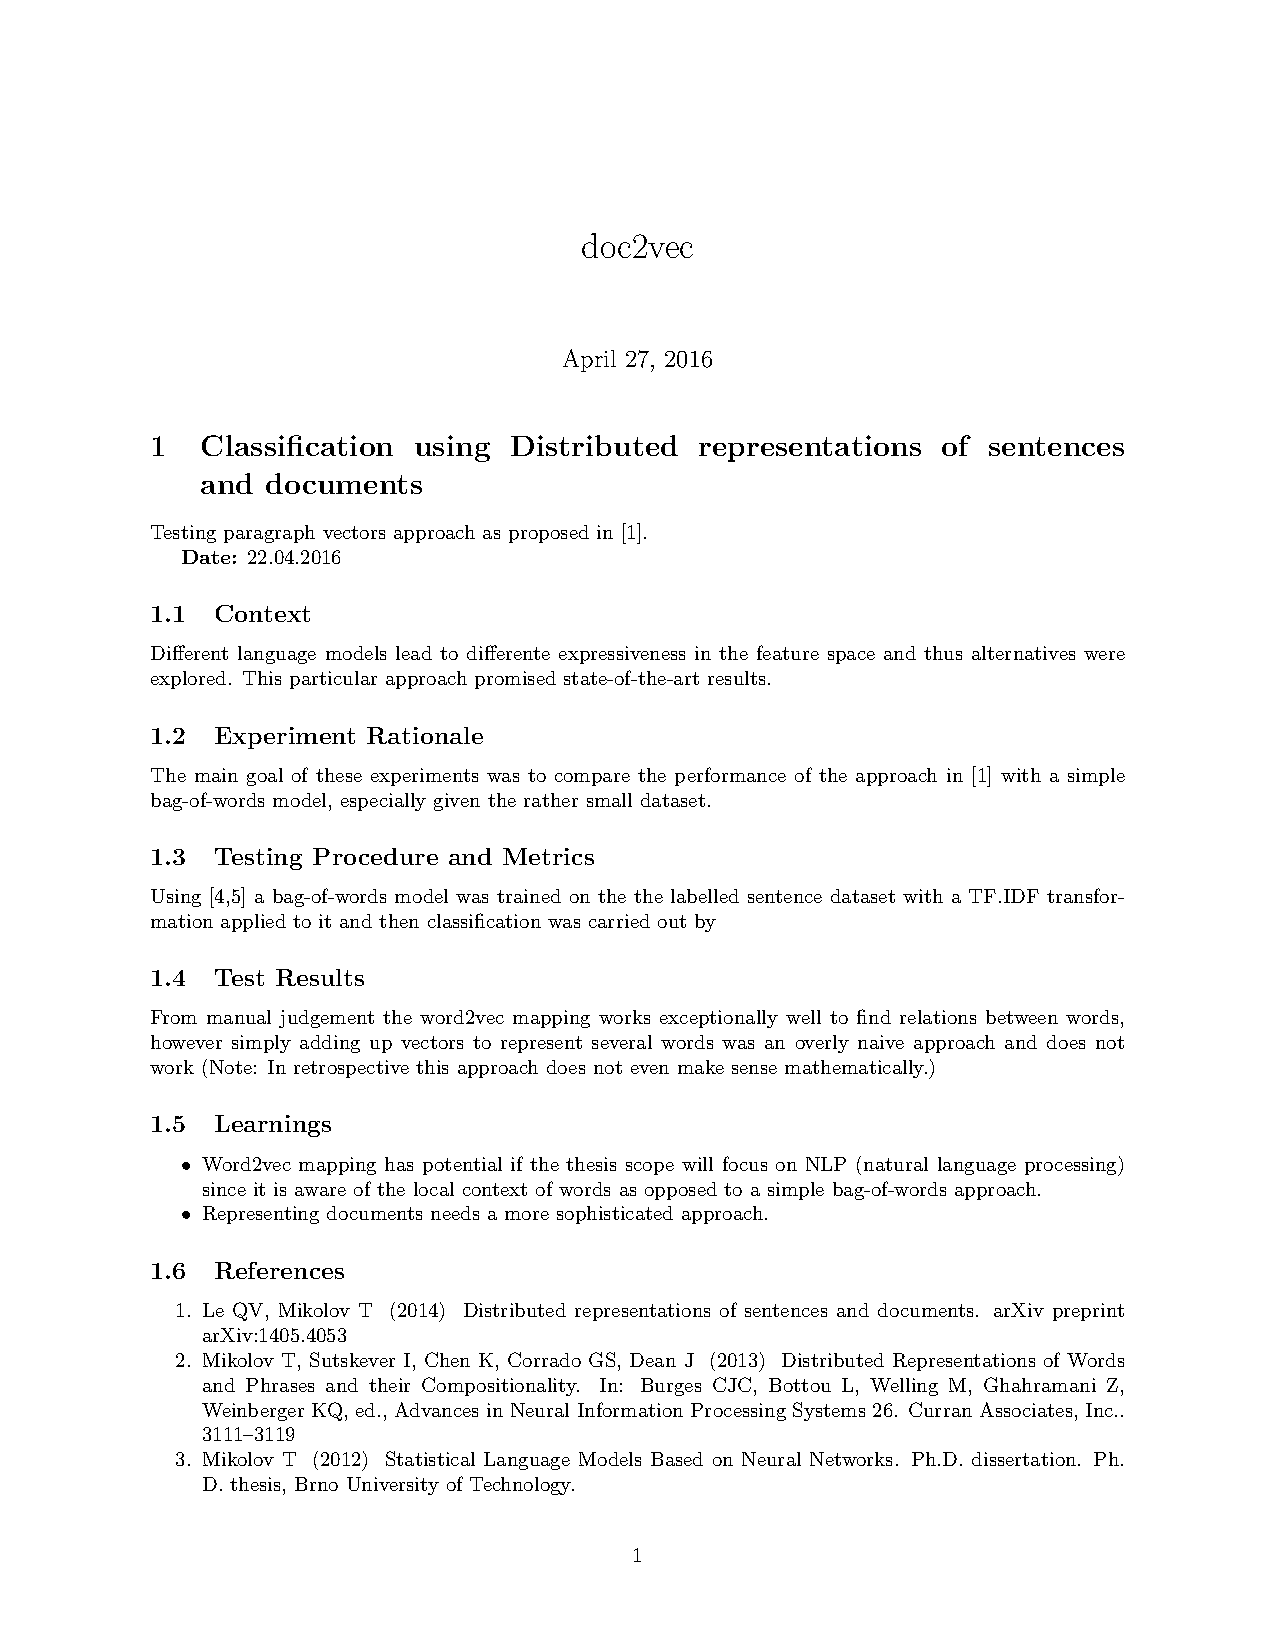
\includepdf[pages=-, offset=75 -75]{appendix/doc2vec.pdf}


\end{document}
